%%
%% MSc Final Graduation Report
%% Based on the ACM "acmart" double-column template (sigconf)
%% Populated from the Research Plan; sections marked [TODO] need
%% post-experiment data, code-derived numbers, or final reflections.
%%
%% Compile with: pdflatex -> bibtex (or just pdflatex twice if using
%% the embedded thebibliography) -> pdflatex -> pdflatex
%%

\documentclass[sigconf,nonacm]{acmart}

%% \BibTeX command to typeset BibTeX logo in the docs
\AtBeginDocument{%
  \providecommand\BibTeX{{%
    Bib\TeX}}}

%% Packages carried over from the research plan + standard thesis tools
\usepackage{tabularx}
\usepackage{multirow}
\usepackage{array}
\usepackage{enumitem}
\usepackage{booktabs}
\usepackage{graphicx}
\usepackage{amsmath}
\usepackage{amssymb}
\usepackage{subcaption}
\usepackage{listings}
\usepackage{xcolor}
\usepackage{tikz}
\usepackage{float}
\usetikzlibrary{positioning, arrows.meta, shapes.geometric, fit}

%% Suppress ACM-specific footers/headers since this is a thesis, not an ACM submission.
\settopmatter{printacmref=false}
\renewcommand\footnotetextcopyrightpermission[1]{}
\pagestyle{plain}

\begin{document}

%%
%% TITLE
%% Finalized title should reflect results once experiments are complete.
%% [TODO] Consider adapting if your strongest finding shifts the framing.
\title{Constraint-Aware Interaction Generator for Synthetic E-commerce data}
\subtitle{An End-to-End pipeline for training and evaluating interaction generators.}

%%
%% AUTHOR INFORMATION
\author{Beau Min}
\email{beau.min@hva.nl}
\affiliation{%
  \institution{Amsterdam University of Applied Sciences}
  \city{Amsterdam}
  \country{The Netherlands}
}

\renewcommand{\shortauthors}{Min}

%%
%% STRUCTURED ABSTRACT
%% [TODO] Replace placeholder Results and Conclusion sentences with your
%%        final numbers and findings once experiments are complete.
\begin{abstract}
Recommender-system simulators rely on synthetic interaction logs whose
fidelity, validity, and downstream utility determine whether
simulation-based studies remain credible. Existing simulators in the
RS-simulation literature are dominated by process-based, agent-based,
statistical, and adversarial approaches, while transformer sequence
modeling has been applied almost exclusively to next-item prediction
rather than full-session generation. This approach bridges the two lines
with a multi-head autoregressive transformer that emits typed
interaction tuples (action type, item, inter-event time) jointly,
embedded in a process-based simulation wrapper and trained on the
Synerise RecSys~2025 retail dataset. Three iterations of the item head
(flat $K$-way softmax, category-hierarchical, and SVD-PQ
token-factored) target the popularity-collapse failure mode of the
flat baseline at successively stronger structural priors, and a
hard-constraint validity layer reports pre- and post-repair violation
rates for three behavioral constraints to keep generation assumptions
auditable. Quality is measured under a multi-axis protocol covering
distributional fidelity, behavioral validity, and downstream utility
(TSTR HR@10 / NDCG@10) against a Markov-style baseline, with five-seed
variance reporting. TODO: Results & Conclusion & Reflection.
\end{abstract}

%% CCS CONCEPTS -- replace with concepts from https://dl.acm.org/ccs/ccs.cfm
\begin{CCSXML}
<ccs2012>
 <concept>
  <concept_id>10002951.10003317</concept_id>
  <concept_desc>Information systems~Recommender systems</concept_desc>
  <concept_significance>500</concept_significance>
 </concept>
 <concept>
  <concept_id>10010147.10010178.10010187</concept_id>
  <concept_desc>Computing methodologies~Neural networks</concept_desc>
  <concept_significance>300</concept_significance>
 </concept>
 <concept>
  <concept_id>10010147.10010257</concept_id>
  <concept_desc>Computing methodologies~Modeling and simulation</concept_desc>
  <concept_significance>300</concept_significance>
 </concept>
</ccs2012>
\end{CCSXML}

\ccsdesc[500]{Information systems~Recommender systems}
\ccsdesc[300]{Computing methodologies~Neural networks}
\ccsdesc[300]{Computing methodologies~Modeling and simulation}

\keywords{recommender systems, synthetic data, simulation, transformer,
interaction generation, evaluation protocol}

\maketitle

%% =====================================================================
\section{Introduction}
\label{sec:introduction}

\subsection{Context}
Recommender systems (RS) are frequently developed and evaluated on static
historical logs. This is practical but methodologically incomplete. When
recommendation policies change, user exposure changes. When exposure changes,
user behavior changes. When behavior changes, future training data changes.
Static snapshots therefore fail to capture the feedback dynamics that emerge
in iterative deployment. Offline evaluation on fixed logs can look convincing
while still missing important behavioral effects that only materialize under
continuous operation. This challenge is repeatedly identified in the
recommender simulation literature as a fundamental reason for interest in
synthetic interaction generation as a methodological
tool~\cite{stavinova2022survey,ekstrand2021simurec,chaney2021challenges}.

\subsection{Problem Statement}
The RS simulation literature is active but methodologically fragmented.
Existing approaches include process-based and framework-oriented
simulators~\cite{bountouridis2019siren,lucherini2021trecs,mcinerney2021accordion},
adversarial and statistical generators~\cite{zhao2021usersim,bobadilla2023ganrs},
and configurable data synthesis tools~\cite{delcarmen2017datacgencars,jakomin2018gids}.
These lines provide important building blocks but also reveal recurring
issues: heterogeneous assumptions, inconsistent metric usage, and weak
comparability across studies~\cite{stavinova2022survey,chaney2021challenges}.

The project context of this thesis is a two-component recommender system
simulator developed at the AUAS Centre for Market Insights (CMI). An arrival
component is already operational, while an interaction generator is the open
problem. The prior implementation couples a first-order Markov chain with an
LSTM that functions as a feature extractor for item ranking, not a learned
sequence generator. The interaction generation is therefore a patchwork of
three mechanisms: a recommender that selects items, a Markov chain that picks
behavior transitions, and hardcoded session logic that glues them together.
There is no single learned model generating coherent interaction sequences
end-to-end. The result is implausible session structures: action sequences
that violate behavioral funnels at rates incompatible with observed data, and
insufficient distributional coverage across the item space.

\subsection{Existing Work}
Sequential recommendation has demonstrated strong performance from transformer
architectures, with SASRec~\cite{kang2018sasrec},
BERT4Rec~\cite{sun2019bert4rec}, and GRU4Rec~\cite{hidasi2015gru4rec}
representing the progression from recurrent to attention-based methods.
However, prediction success does not automatically transfer to synthetic
interaction generation. Generator design requires distinct choices around
output structure, validity constraints, temporal handling, and evaluation
criteria. A more detailed treatment of related work is given in
Section~\ref{sec:background}.

\subsection{Research Gap}
Across the RS simulation literature reviewed for this thesis, no work that
uses a non-LLM autoregressive transformer as the primary architecture for
generating enriched interaction event logs was identified. The RS simulation
branch relies entirely on process-based, agent-based, statistical, or
adversarial approaches, while the sequential recommendation branch applies
transformers exclusively to next-item prediction, not to session generation.
This thesis is positioned at the intersection of these two lines.

\subsection{Proposal and Research Questions}
This thesis proposes a hybrid architecture: a multi-head autoregressive
transformer embedded in a process-based simulation wrapper, generating typed
event sequences with explicit hard constraints. The contribution is both
\emph{technical}, in the form of a multi-head autoregressive architecture for
typed event tuple generation, and \emph{methodological}, a reproducible
evaluation protocol for simulator quality claims along fidelity, validity,
and downstream utility.

The work is guided by the following main research question and sub-questions:
\begin{quote}
\textit{How and to what extent can a constraint-aware autoregressive
transformer interaction generator produce synthetic interaction logs with
high fidelity, validity, and downstream utility for recommender-system
training and evaluation?}
\end{quote}

\begin{itemize}[leftmargin=*]
  \item \textbf{SQ1:} How should interactions be formally defined for
    simulation purposes, covering event fields, temporal structure, and
    session dependencies?
  \item \textbf{SQ2:} What architectural properties does an interaction
    generator need to capture realistic interaction dynamics, including
    sequential dependence, action--item coherence, and temporal structure?
  \item \textbf{SQ3:} Which generator implementations and baseline policy
    are feasible within thesis scope for a fair and executable comparison?
  \item \textbf{SQ4:} Which evaluation protocol makes ``better than
    baseline'' falsifiable and reproducible?
\end{itemize}

\subsection{Contributions}
The main contributions of this work are:
\begin{enumerate}[leftmargin=*]
  \item A multi-head autoregressive transformer architecture for typed event
    tuple generation, with factored heads for action type, item, and
    inter-event time.
  \item A reproducible, multi-axis evaluation protocol covering fidelity,
    validity, and downstream utility, with variance reporting across seeds.
\end{enumerate}

\subsection{Report Structure}
Section~\ref{sec:background} presents the theoretical background, state of
the art, stakeholder analysis, and AI considerations.
Sections~\ref{sec:method-design}--\ref{sec:method-evaluation} detail the
methodology. Section~\ref{sec:results} reports the results.
Section~\ref{sec:discussion} discusses them, and
Section~\ref{sec:conclusion} concludes.

%% =====================================================================
\section{Background}
\label{sec:background}

\subsection{Theoretical Foundations}
\label{sec:theory}

\subsubsection{Interaction as Typed Temporal Event Sequences}
Across the RS simulation papers reviewed for this work, ``interaction'' is
more than a $\langle$user, item, rating$\rangle$ tuple. Accordion models
events as
% Mooie hbox
\textit{(time, user, item, outcome)} with visit
dynamics~\cite{mcinerney2021accordion}. UserSim models sequential user
behavior conditioned on prior interactions~\cite{zhao2021usersim}. SIREN and
T-RECS model iterative, stateful user--item processes over
time~\cite{bountouridis2019siren,lucherini2021trecs}. DataGenCARS formalizes
context as a generated part of the interaction
record~\cite{delcarmen2017datacgencars}. This convergence of evidence across
different simulator families supports a two-level interaction definition:
event-level typed tuples grouped into sessions, with user state carried
across sessions via history. This definition directly motivates the
multi-head prediction architecture described in
Section~\ref{sec:method-model}.

\subsubsection{Sequential Dependence as a Modeling Requirement}
Realistic interaction sequences are not independent and identically
distributed events. A user who views an item, then adds it to cart, then
removes it, exhibits session-level dependence that first-order Markov chains
cannot capture reliably. Chaney~\cite{chaney2021challenges} identifies missed
behavioral dependencies as a central simulation validity risk, particularly
when models make implicit IID assumptions that the real data does not
support. Accordion demonstrates that temporal process modeling changes
long-term simulation effects substantially~\cite{mcinerney2021accordion}.
This motivates sequence-capable generators over IID-only approaches and
justifies the autoregressive design of the proposed transformer.

\subsubsection{Adversarial Generation: Utility and Risk Tradeoffs}
GAN-based user simulators provide utility-oriented
evidence~\cite{zhao2021usersim,bobadilla2023ganrs} but carry well-documented
limitations. Creswell et al.~\cite{creswell2018gan} document mode collapse
and optimization instability as structural GAN risks, while Figueira and
Vaz~\cite{figueira2022survey} note persistent evaluation ambiguity. For
discrete sequential generation specifically, gradient flow through discrete
tokens requires additional workarounds that compound architectural
complexity. Autoregressive transformers with softmax output heads handle
discrete token generation natively, which is a structural advantage for the
interaction generation task.

\subsubsection{Multi-Axis Evaluation as a Scientific Requirement}
Jordon et al.~\cite{jordon2022synthetic} argue that utility-only validation
is insufficient: synthetic data that enables good downstream models may still
be statistically implausible at the distributional level. Figueira and
Vaz~\cite{figueira2022survey} reinforce that single-metric evaluation is
systematically incomplete. Stavinova et al.~\cite{stavinova2022survey}
document heterogeneous and non-comparable metrics across simulators.
\subsubsection{Reproducibility and Assumption Explicitness}
T-RECS emphasizes multi-run confidence intervals and repeated-run variance
analysis as scientific requirements for simulation
research~\cite{lucherini2021trecs}. SimuRec identifies reproducibility as a
missing standard across the community~\cite{ekstrand2021simurec}.
Chaney~\cite{chaney2021challenges} argues that simulation conclusions are
only credible when modeling assumptions are stated explicitly and tested
empirically. This thesis operationalizes these requirements through fixed
random seeds, deterministic preprocessing, and a hard-constraint validity
layer that makes generation assumptions explicit and measurable. Results are
reported across five seeds to surface variance.

\subsection{State of the Art}
\label{sec:sota}

\subsubsection{Recommender System Simulation Landscape}
Stavinova et al.~\cite{stavinova2022survey} document heterogeneous
simulators, missing standardized head-to-head comparisons, and weak universal
quality-control methodologies. SimuRec~\cite{ekstrand2021simurec} identifies
the absence of shared standards as a community-level gap and motivates the
need for more systematic evaluation frameworks. Heterogeneous evaluation
practices mean that results across existing simulators are rarely directly
comparable, undermining cumulative scientific progress.

Process-based and framework-oriented simulators form one branch of the
literature. SIREN~\cite{bountouridis2019siren} demonstrates the simulation of
longitudinal recommender effects in online news environments, with explicit
user--system feedback dynamics modeled over time.
T-RECS~\cite{lucherini2021trecs} lowers the barrier to long-horizon RS
simulation through a modular, agent-based design and multi-run confidence
intervals for variance-aware analysis. Accordion~\cite{mcinerney2021accordion}
models user visits as inhomogeneous Poisson processes with marked events,
demonstrating that explicit temporal process modeling substantially changes
simulated long-term interactive effects. These tools establish the
system-level context this thesis operates within, while leaving event-level
interaction generation largely to domain assumptions or simplified
behavioral rules.

Adversarial and statistical generation form a second branch.
UserSim~\cite{zhao2021usersim} applies a supervised GAN to simulate user
behavior for offline reinforcement learning over recommender systems.
Bobadilla et al.~\cite{bobadilla2023ganrs} generate parameterized
collaborative filtering datasets via GAN for configurable benchmark
construction. DataGenCARS~\cite{delcarmen2017datacgencars} and Jakomin et
al.~\cite{jakomin2018gids} provide configurable statistical generators for
context-aware and stream-based interaction data.

Evaluation challenges are a cross-cutting concern. Figueira and
Vaz~\cite{figueira2022survey} identify that single-metric evaluation is
insufficient for synthetic data claims. Jordon et
al.~\cite{jordon2022synthetic} articulate that utility-only validation does
not guarantee distributional fidelity. Lu et al.~\cite{lu2024review} identify
missing standardized evaluation tools across the synthetic data generation
field. This convergent critique motivates the multi-axis evaluation design
of this thesis.

\subsubsection{Sequential Modeling and Transformers}
Transformers have proven dominant for next-item prediction in sequential
recommendation. SASRec~\cite{kang2018sasrec} established causal
self-attention for sequential RS, demonstrating that attention-based models
substantially outperform Markov chains and RNNs on next-item prediction
benchmarks. BERT4Rec~\cite{sun2019bert4rec} extended this with masked
training objectives for bidirectional context modeling.
GRU4Rec~\cite{hidasi2015gru4rec} is the canonical RNN predecessor that
transformers have consistently outperformed on longer sequences.

However, next-item prediction and synthetic interaction log generation are
distinct tasks. Prediction asks: given history, what item comes next?
Generation asks: produce a full, distributionally realistic interaction
session from scratch. The output structure, evaluation criteria, and success
measures differ fundamentally. This thesis applies transformer sequence
modeling to generation, not prediction; the architectural transfer is
strongly motivated by evidence but cannot be assumed automatic. Generated
logs require additional evaluation along fidelity and validity axes that
next-item accuracy alone does not capture.

\subsection{Stakeholder Analysis}
\label{sec:stakeholders}

\paragraph{Academic supervisor (Diptish Dey, CMI).}
Diptish Dey is the primary owner of this project. His stake is in a working,
validated interaction generator that integrates with the existing arrival
simulator. Timely delivery and a defensible evaluation methodology matter to
him because the simulator is part of ongoing research at CMI.

\paragraph{CMI research group.}
The broader CMI research group has a practical stake in the technical
output. Colleagues working on related projects stand to benefit from a
reusable simulator component and a documented evaluation protocol they can
apply or extend without having to rebuild from scratch.

\paragraph{CMI researchers (operator end-user).}
The immediate end-user of the deliverable is a CMI researcher who runs the
simulator: configures a generation experiment, executes the pipeline, and
inspects the resulting metrics. Their stake is operational rather than
methodological. They benefit from a configuration-driven entry point, a
deterministic re-run path on a fixed seed, and metrics output that does not
require code changes to interpret. Decisions made for this end-user
include the configuration-file-driven experiment runner, the four-stage
artefact-based pipeline (so any single stage can be re-run without
re-running its predecessors), and a single shared evaluation harness for
both generators so cross-generator comparisons require no per-experiment
glue code.

\paragraph{Recommender systems research community.}
The research community's interest is in reusable evaluation protocols,
open-dataset compatibility, and reproducible baselines that support
cumulative scientific progress.

\paragraph{Dataset provider (Synerise / RecSys 2025 challenge).}
Synerise's interest is in demonstrating the richness and utility of their
publicly released dataset. As the dataset is publicly released under
challenge terms, Synerise has no active supervisory or evaluative role in
this project.

\paragraph{Downstream users of the recommender system.}
The behavioral patterns in the Synerise logs represent real user
populations. These anonymous users have an interest in synthetic data not
amplifying distributional biases present in the real logs, such as
popularity skew. This interest is addressed through bias metrics
(Jensen--Shannon divergence on action distributions, item coverage) reported
as part of the fidelity evaluation. The Synerise logs represent real
people's shopping behavior; this research neither re-identifies nor profiles
any individual, in accordance with the legal requirements detailed in
Section~\ref{sec:method-requirements}.

\paragraph{Conflicting interests and prioritization.}
The stakeholder interests above are largely aligned but diverge on two
points. First, the academic supervisor's interest in timely delivery is in
tension with the research community's interest in broad generalizability. A
more extensive comparison portfolio, covering additional baselines such as
GRU- or GAN-based generators, would strengthen the community contribution
but risks overrunning the thesis timeline. This tension is resolved in
favor of the supervisor's constraint: scope is fixed to a single transformer
versus Markov chain comparison, with extensions explicitly identified as
future work. Second, Synerise's interest in showcasing dataset richness is
in tension with downstream users' interest in not amplifying bias. A
generator optimized purely for distributional fidelity will faithfully
reproduce whatever popularity skew is present in the training data. This
tension is resolved by including explicit bias metrics in the fidelity
evaluation rather than treating fidelity-to-data and fairness-to-users as
equivalent goals.

\subsection{Current Situation}
\label{sec:current-situation}
The interaction generator currently in use within the CMI simulator is a
patchwork of three independent mechanisms rather than a single learned
sequence model: a recommender selects items, a first-order Markov chain
selects action transitions, and hardcoded session logic glues the two
together (Section~\ref{sec:introduction}). The result, as documented in
the same section, is implausible session structures and insufficient
distributional coverage across the item space. The proposed transformer
generator described in Section~\ref{sec:method-model} replaces all
three mechanisms with one autoregressive model whose factored heads
emit action, item, and inter-event time jointly, and whose
distributional and behavioral fidelity is evaluated against the
existing Markov-style mechanism using the protocol of
Section~\ref{sec:method-eval}.

\subsection{AI Considerations}
\label{sec:ai-considerations}

\subsubsection{Suitability of a Learned Model}
Rule-based approaches to interaction generation, such as handcoded Markov
chains with manually specified legal transitions, require exhaustive
elicitation of every valid behavioral path and cannot generalize to unseen
contexts or long-range session dependencies. Learned models extract
transition probabilities from data and capture dependencies that fixed
rules cannot express~\cite{chaney2021challenges,mcinerney2021accordion}. The
case for a learned model over handcoded rules follows from this.

\subsubsection{Autoregressive vs.\ Non-Autoregressive Generation}
Autoregressive generation is not the only design option for learned sequence
models. Parallel or non-autoregressive generation methods produce all output
tokens simultaneously, offering higher throughput. However, parallel
generation requires conditional independence assumptions across output
positions that are incompatible with the behavioral dependencies documented
in the literature: a generated action type must condition on prior actions,
and a generated item must condition on the current action type. Violating
these dependencies at generation time would undermine the validity of the
constraint layer and the fidelity of the output
log~\cite{chaney2021challenges}. Autoregressive generation is therefore the
appropriate choice for this task, with throughput as an acknowledged
tradeoff.

Among learned approaches, a transformer architecture is preferred over
simpler sequence models. The factored multi-head design enables joint
action--item--time modeling, and self-attention captures long-range session
dependencies more effectively than first-order Markov chains or other
recurrent
architectures~\cite{kang2018sasrec,sun2019bert4rec,hidasi2015gru4rec}.

\subsubsection{Degree of Automation and Societal Considerations}
Full automation of the generation pipeline is appropriate for this use case
because the output is synthetic training data rather than decisions
affecting real users directly. No human-in-the-loop is required at
generation time. However, the hard-constraint validity layer makes the
automation explicit and auditable: generation assumptions are documented as
constraint rules extracted from real data, and violations are counted and
reported.

Recommender systems trained on synthetic interaction data influence what
products, content, and services real users are exposed to at scale. If the
generator systematically amplifies distributional biases present in the
training data, downstream recommenders trained on that data may entrench
those patterns further. The most significant risk is feedback loop
amplification: a biased generator produces biased training data, which
trains a biased recommender, which produces biased interaction logs, which
are used to retrain the generator. This risk is not fully neutralized by
bias reporting alone, measuring a problem does not resolve it. The
mitigation in this thesis is therefore scoped honestly: bias metrics are
reported to make the problem visible and quantifiable, enabling downstream
researchers and practitioners to make informed decisions about whether and
how to deploy synthetic data produced by this pipeline.

%The research is nonetheless justified. The alternative, continued reliance
%on static historical logs for recommender evaluation, carries its own
%unacknowledged biases and feedback dynamics. A transparent, auditable
%synthetic generator with documented bias characteristics is a more
%controllable research instrument than an unexamined historical log.

%% =====================================================================
\section{Methodology: Research Design}
\label{sec:method-design}

\subsection{Research Approach}
The project follows a design-and-evaluate methodology across three phases:
specification, modeling, and evaluation. The specification phase formalizes
the interaction schema, simulator interfaces, and evaluation protocol. The
modeling phase implements the Markov baseline and transformer generator.
The evaluation phase runs the fidelity–validity–utility protocol with
statistical reporting.

\subsection{Experimental Setup}
All training and evaluation runs are executed on a single workstation
with one NVIDIA GeForce RTX 4070~Ti GPU (12\,GB VRAM, driver
$595.71.05$), running CachyOS Linux (kernel $7.0.3$) with CUDA $13.2$. Python dependencies are pinned in
\texttt{uv.lock} and resolved by the \texttt{uv} package manager; the
versions relevant to the experiments are PyTorch~$2.11.0$, NumPy~$2.4.4$,
Polars~$1.39.3$, and pandas~$3.0.2$.

Multi-seed reporting uses five consecutive integer seeds starting at
$42$, i.e.\ $\{42, 43, 44, 45, 46\}$. The same seed set is reused for
final evaluation (\texttt{final\_eval\_seeds} in the configuration). Preprocessing, cleaning, sessionization, and split steps depend only on the input parquets and
the configured cutoffs, and produce byte-stable
output artefacts.


%% =====================================================================
\section{Methodology: Requirements}
\label{sec:method-requirements}

\subsection{Legal Requirements}
The primary dataset is the Synerise RecSys 2025 dataset, released publicly
under the RecSys 2025 challenge terms. The dataset consists of anonymized
behavioral event logs with no personally identifiable information (PII).
Processing anonymized behavioral data for academic research is permissible
under the scientific research exemption of the EU General Data Protection
Regulation (GDPR, Art.~89)~\cite{gdpr2016}. Generated synthetic data carries
minor re-identification risk: item-ID vocabulary capping reduces the item space
to a top-$K$ vocabulary, and all outputs are population-level statistics
rather than individual records.

\subsection{Ethical Requirements}
Synthetic interaction data trained on real behavioral logs inherits the
distributional properties of that data, including popularity skew, temporal
selection effects, and potential demographic proxy
signals~\cite{jordon2022synthetic,chaney2021challenges}. This risk is
acknowledged and is made visible by reporting bias metrics as part of the
fidelity evaluation: Jensen--Shannon divergence over the action-type
distribution and item coverage are both reported. Reporting does not
eliminate the inherent bias in the training distribution, but does make the
inherited skew transparent.

The generation pipeline must not be used for individual-level profiling or
decisions. Use is restricted to aggregate training data generation. The
explicit hard-constraint layer documents and enforces generation assumptions.

\subsection{Organizational Requirements}
The project is conducted by a single developer within the thesis timeline.
The deliverable is an academic thesis document and a demonstrator pipeline.
Weekly supervision meetings with supervisor Diptish Dey provide structured checkpoints.

\subsection{Functional Requirements}
The generator must produce typed event tuples conforming to the schema in
Table~\ref{tab:schema}: (\texttt{user\_id}, \texttt{session\_id},
\texttt{action\_type}, \texttt{item\_id}, \texttt{delta\_t}). The five-action
vocabulary of the Synerise dataset must be respected. Session structure must
follow observed behavioral conventions: sessions begin on an arrival signal
from the arrival simulator and terminate on an EOS token or a session length
cap. The interface contract accepts the arrival simulator's output as input
and produces a log conforming to the schema. All generated sessions must
pass through the validity layer before output.

\subsection{Technical Requirements}
The model must be trainable on a single GPU within the timeline. Vocabulary
capping ensures softmax tractability and prevents Out-Of-Memory errors by limiting the item space to the
top-$K$ most frequent items. Evaluation infrastructure must be deterministic:
fixed random seeds, configuration-driven experiment runs, and all
hyperparameters logged.

The evaluation pipeline must support reproducible execution across multiple
random seeds. The generator must be deployable within the containerized
simulation environment alongside the arrival simulator.

%The evaluation protocol imposes the following measurement constraints.
%Fidelity is assessed via four metrics: Jensen--Shannon divergence over the
%action-type distribution (JSD), the two-sample Kolmogorov--Smirnov statistic
%over session length distributions (KS), L1 distance over the action bigram
%transition matrix, and L1 distance over the item bigram transition matrix
%restricted to item-bearing events (\texttt{product\_buy},
%\texttt{add\_to\_cart}, \texttt{remove\_from\_cart}). Validity is assessed
%via three constraint violation rates: illegal action transition rate,
%timestamp monotonicity violation rate, and purchase-without-prior-exposure
%rate. Both pre- and post-constraint-layer rates must be reported. Downstream
%utility is assessed via HR@10 and NDCG@10 under the TSTR paradigm. All
%metrics must be reported as mean and standard deviation across five random
%eeds. The transformer generator (TSTR-T) must outperform the Markov
%baseline (TSTR-M) on both HR@10 and NDCG@10 for the utility claim to be
%considered confirmed. Improvement on one metric only is treated as
%inconclusive.

\subsection{Validation of Requirements}
\label{sec:requirements-validation}
The five categories of requirements above were validated as follows.

\paragraph{Legal.}
The Synerise RecSys~2025 dataset is distributed under the MIT licence
attached to the public release repository, which permits use, modification,
and redistribution subject only to inclusion of the copyright notice and
disclaimer. No separate data-use agreement is associated with the release.
The pipeline therefore complies with the legal basis named in
Section~\ref{sec:method-requirements} by (i) operating only on the
publicly released parquets, (ii) processing no PII fields
(\texttt{client\_id} and \texttt{sku} are opaque integers, see
Section~\ref{sec:method-data}), and (iii) restricting all reported
outputs to population-level aggregates so that no individual-level
record produced by the pipeline is published.

\paragraph{Ethical.}
The ethical requirement to make bias inheritance visible rather than
silent was validated by (i) computing the bias-metric group (item
coverage, popularity JSD, $\Delta$Gini) on every generated batch as
part of the standard fidelity evaluation and (ii) using these metrics
as a development signal during model iteration. Two
hyperparameters were added to the pipeline in direct response to bias
readings: an inverse-frequency item-CE weight
(\texttt{item\_loss\_freq\_weight\_alpha}) and a Menon-style category
logit adjustment (\texttt{cat\_logit\_adj\_tau}) \cite{menon2021longtaillearninglogitadjustment}.% Both are off by
%default and were introduced when popularity-JSD and Gini-delta
%diagnostics indicated head-only collapse on a candidate iteration.
%Bias reporting therefore did not remain a passive disclosure; it
%shaped the design of the model itself.

\paragraph{Organizational.}
The timeline constraint was validated by
delivery against the project planning held on the supervision team's
shared planning board, with weekly check-ins with supervisor Diptish Dey throughout
the project. %Personal notes were kept for the more substantive meetings
%(timestamped by their last-edit metadata); no formal minutes were
%produced because not every meeting carried decisions worth minuting.

\paragraph{Functional.}
The functional requirements decompose into a behavioral contract and a
schema contract. The behavioral contract, legal action transitions,
timestamp monotonicity, and purchase-without-prior-exposure, is
validated automatically at generation time by the constraint
validity layer (\texttt{evaluation/validity\_checker.py},
Section~\ref{sec:validity}); both pre- and post-repair violation rates
are reported in Section~\ref{sec:validity-metrics}, which makes the
constraint check measurable.
%The schema
%contract from Table~\ref{tab:schema} is currently validated only
%implicitly: downstream stages crash on a schema mismatch, but no
%explicit schema assertion is wired in. A small \texttt{assert}-level
%schema check on the generator's output parquet is identified as a
%follow-up [TODO~--~add explicit schema assertions or a pydantic /
%\texttt{polars.Schema} check on the generation log].

\paragraph{Technical.}
The technical requirements were validated by direct measurement on the
hardware described in Section~\ref{sec:method-design}. GPU memory stayed
below $4$\,GB during training and below $6$\,GB during evaluation on the
$12$\,GB RTX~4070~Ti, so the single-GPU training requirement is met with headroom. Determinism is validated by
re-running the preprocessing pipeline against the same input parquets
and observing byte-stable output artefacts across runs; multi-seed
reproducibility is validated by the five-seed evaluation protocol
(Section~\ref{sec:tstr}).
%The deployability-alongside-the-arrival-simulator
%requirement is met by reading the arrival simulator's output as the
%generator's input contract; an explicit end-to-end throughput
%measurement against the arrival simulator was not performed and is
%identified as future work.

%% =====================================================================
\section{Methodology: Data}
\label{sec:method-data}

\subsection{Dataset Description}
The experiments use the Synerise RecSys 2025 retail e-commerce dataset. The raw
release contains $225{,}224{,}262$ timestamped interaction events collected over
168 days, from 23~June~2022 to 8~December~2022, together with a product metadata
table. The interaction schema comprises five event types: \texttt{page\_visit},
\texttt{search\_query}, \texttt{add\_to\_cart}, \texttt{remove\_from\_cart}, and
\texttt{product\_buy}. The release used in this thesis therefore consists of five
event parquet files and one \texttt{product\_properties} parquet file, rather
than six event files.

The raw action distribution is imbalanced toward browsing activity, as
shown in Table~\ref{tab:raw-action-distribution}. Page visits account for
$88.56\%$ of all logged events, while purchases account for only $1.03\%$. This
asymmetry is important for both modeling and evaluation: the generator must
learn realistic transition behavior in a corpus where low-value, high-frequency
browsing events dominate the event stream. The temporal structure of this stream
is shown in Figure~\ref{fig:weekly-event-volume}, where weekly event volume per
type is plotted together with the train/validation/test split boundaries used by
the pipeline. Event volume rises substantially over the observation window, and
the held-out periods overlap with the densest portion of the corpus.

\begin{table}[t]
    \centering
    \caption{Raw action distribution in the Synerise RecSys 2025 dataset.}
    \label{tab:raw-action-distribution}
    \begin{tabular}{lrr}
        \hline
        Action type                 & Count           & Share    \\
        \hline
        \texttt{page\_visit}        & 199{,}451{,}980 & 88.56\%  \\
        \texttt{search\_query}      &  13{,}223{,}769 &  5.87\%  \\
        \texttt{add\_to\_cart}      &   7{,}541{,}117 &  3.35\%  \\
        \texttt{remove\_from\_cart} &   2{,}688{,}894 &  1.19\%  \\
        \texttt{product\_buy}       &   2{,}318{,}502 &  1.03\%  \\
        \hline
        Total                       & 225{,}224{,}262 & 100.00\% \\
        \hline
    \end{tabular}
\end{table}

\begin{figure}[t]
    \centering
    \includegraphics[width=\linewidth]{images/data/weekly_event_volume.png}
    \caption{Weekly event volume by type on the post-preprocessing corpus, with
    train/validation and validation/test split boundaries marked. Event volume is
    non-stationary across the observation window; the held-out splits lie in the
    highest-volume period.}
    \label{fig:weekly-event-volume}
\end{figure}

The product metadata table contains $1{,}534{,}050$ rows with four fields:
\texttt{sku}, \texttt{category}, \texttt{price}, and \texttt{name}. No null
values are present in these columns. The catalog contains $6{,}912$ distinct
categories and 100~price buckets, and metadata coverage for training SKUs is
complete. This makes the dataset suitable for feature-augmented sequence
modeling and for extracting item-category constraint structure from the
training split.

The item distribution is strongly long-tailed. Under the realized training split
used by the pipeline, $9{,}338{,}690$ item-bearing events span $1{,}305{,}867$
unique SKUs. Table~\ref{tab:vocab-coverage-K} reports the vocabulary size $K$
needed to cover a target fraction of training item-bearing events, and
Figure~\ref{fig:vocabulary-coverage} visualizes the same coverage curve along
with the embedding-table memory cost as $K$ grows and the long-tail bucket
breakdown. Three orders of magnitude separate the $K$ required for $50\%$
coverage from the $K$ required for $99\%$ coverage.
%This Zipf-like behavior
%makes the choice of item vocabulary size a central design decision rather than
%an implementation detail.
The long-tail structure recurs per action type:
Figure~\ref{fig:sku-action-loglog} shows that \texttt{add\_to\_cart},
\texttt{remove\_from\_cart}, and \texttt{product\_buy} all follow the same
approximate power-law shape over their respective SKU ranks, with strongly
correlated frequencies across action types.
%-- which justifies a single shared
%item embedding rather than separate per-action vocabularies.

\begin{table}[t]
    \centering
    \caption{Vocabulary size $K$ needed to cover a target fraction of training
    item-bearing events. The realized pipeline cap of $K = 200{,}000$ covers
    $71.71\%$.}
    \label{tab:vocab-coverage-K}
    \begin{tabular}{lr}
        \hline
        Target coverage & $K$ (number of SKUs) \\
        \hline
        50\%            &      45{,}456        \\
        80\%            &     338{,}307        \\
        90\%            &     654{,}304        \\
        95\%            &     887{,}771        \\
        99\%            &  1{,}212{,}481       \\
        \hline
    \end{tabular}
\end{table}

\begin{figure}[t]
    \centering
    \includegraphics[width=\linewidth]{images/data/vocabulary_coverage.png}
    \caption{Vocabulary analysis on the training split. Left: cumulative coverage
    and UNK rate as a function of $K$ on a log scale, with the configured
    pipeline cap and 80\%/90\%/95\% reference points marked. Middle: float32
    embedding-table size in MB versus $K$ for embedding dimensions
    $d \in \{64, 128, 256\}$. Right: the long-tail breakdown of SKU frequency,
    contrasting the share of SKUs against the share of events they account for.}
    \label{fig:vocabulary-coverage}
\end{figure}

\begin{figure}[t]
    \centering
    \includegraphics[width=\linewidth]{images/data/sku_action_loglog.png}
    \caption{Per-action-type SKU distributions on the training split. Left:
    pairwise SKU set overlaps. Right: log--log frequency curves for
    \texttt{add\_to\_cart}, \texttt{remove\_from\_cart}, and
    \texttt{product\_buy}, all showing the same approximate power-law decay.}
    \label{fig:sku-action-loglog}
\end{figure}

The interaction stream is not only long-tailed at the item level; it is also
structured at the session level. Following a priority-based labelling
(\texttt{purchase} $\succ$ \texttt{cart} $\succ$ \texttt{search} $\succ$
\texttt{browse}, where each session is labelled by the highest-priority event it
contains), the training split decomposes into $2.0\%$ pure browse sessions,
$32.8\%$ search-only sessions, $45.2\%$ sessions that reach the cart but not
checkout, and $19.9\%$ purchase sessions. Figure~\ref{fig:session-taxonomy}
visualizes this distribution alongside the implied session-level conversion
funnel ($100\% \rightarrow 98.0\% \rightarrow 65.2\% \rightarrow 19.9\%$), and
$26.2\%$ of training users complete at least one purchase.

\begin{figure}[t]
\centering
\includegraphics[width=\linewidth]{images/data/session_taxonomy.png}
\caption{Session type taxonomy and conversion funnel on the training split.
Sessions are labelled by their highest-priority event. The funnel makes explicit
that purchase-bearing sessions are a one-in-five minority that any session
generator must reproduce in the right proportion rather than collapse into the
dominant browse/search/cart modes.}
\label{fig:session-taxonomy}
\end{figure}

The dataset is well-suited for evaluating interaction generation
because it contains temporally ordered event stream, as well as a
domain-specific behavioral funnel spanning browsing, search, cart management,
and purchase. All the while, the constraints extracted in this thesis are
retail-specific. The resulting legality rules, exposure prerequisites, and
validity checks are therefore  conventions of e-commerce
interaction data, not as domain-agnostic behavioral rules that would
automatically transfer to settings such as media, news, or social feeds.

\subsection{Preprocessing Pipeline}
The preprocessing pipeline is implemented in \texttt{preprocess.py} and
\texttt{ingestion/dataset.py} , and it consists of six main stages.

\begin{enumerate}
    \item \textbf{Schema normalization.}
    The five raw event parquet files are merged into a unified interaction table
    with a shared schema over \texttt{client\_id}, \texttt{timestamp},
    \texttt{event\_type}, and \texttt{sku}. Product metadata is then joined onto
    item-bearing events, adding category and price information from
    \texttt{product\_properties}. This provides a consistent event stream for both
    session construction and downstream feature extraction.

    \item \textbf{Deduplication and timestamp cleanup.}
    Exact duplicate item-bearing events are removed when they share the same
    \texttt{client\_id}, timestamp, and SKU. Interactions with the same user and
    timestamp but different SKUs are retained, since they plausibly correspond to
    multi-item basket actions or simultaneous checkout events. This step removes
    $161{,}673$ exact duplicates from \texttt{add\_to\_cart}, $153{,}675$ from
    \texttt{remove\_from\_cart}, and $380{,}923$ from \texttt{product\_buy}.
    Timestamps are also checked against the dataset bounds (23~June~2022 to
    8~December~2022).

    \item \textbf{Sessionization.}
    User timelines are segmented with a 30-minute inactivity threshold. This
    choice was decideed against the observed gap distribution. Figure~\ref{fig:inter-event-gaps} shows
    the distribution of all within-user inter-event gaps in the
    post-preprocessing corpus, along with the CDF zoomed into the 0-60-minute
    window where any reasonable sessionization threshold must sit. The CDF is
    essentially flat in the 20 to 45-minute range, so the threshold's exact value
    has only a minor effect on the fraction of gaps it cuts.
    Table~\ref{tab:sessionization-sensitivity} quantifies this, varying the
    threshold across $\{20, 30, 45\}$ minutes changes the number of sessions by
    less than $5.5\%$ while preserving median and tail percentiles.
    Figure~\ref{fig:sessionisation-sensitivity} shows the same sensitivity
    analysis visually, together with the session-length CDF and the bucketed
    length distribution under the chosen 30-minute threshold. Sessions containing
    only \texttt{page\_visit} events are removed afterward because they provide
    no item signal and zero of such sessions remain in the final preprocessed corpus.

    \item \textbf{Time-aware split by session start.}
    Train/validation/test assignment is determined by session start time
    rather than individual event time, and rather than by user or by
    random shuffle. The session-start choice avoids in-session leakage:
    a per-event time split would place events of the same session on
    both sides of the boundary, leaking the session-prefix signal that
    the generator is supposed to learn. The time-based choice is
    preferred over a user-based or random split because the deployment
    regime of the simulator is forward-in-time, the generator is
    expected to produce sessions for the period after the training
    window, not for held-out users sampled uniformly from the same
    period, and because a random event-level shuffle would leak both
    temporal and intra-session structure simultaneously. Sessions
    starting before 15~November~2022 are assigned to training, sessions
    starting from 15~November to 1~December~2022 to validation, and
    sessions starting on or after 1~December~2022 to test. The cutoffs
    partition the 168-day observation window into roughly $145/16/8$
    days and place the densest, behaviorally distinct
    late-season traffic (the Black Friday and early holiday-shopping
    period) on the held-out side, so the validation and test splits
    function as a forward-in-time test. The split itself is deterministic given
    the configured cutoffs and involves no randomness, so it
    contributes nothing to the seed-to-seed variance reported in
    Section~\ref{sec:eval-setup}. The realized split sizes are reported
    in Table~\ref{tab:preprocessed-splits}.

    \item \textbf{Vocabulary capping.}
    The item vocabulary is truncated to the most frequent SKUs in the training
    split. The configured value is $K = 200{,}000$, which corresponds to
    $199{,}999$ explicit SKU entries plus a shared zero index used for padding,
    non-item events, and out-of-vocabulary items. Under the realized
    session-start training split, this vocabulary covers $71.71\%$ of training
    item-bearing events, a training OOV rate of $28.29\%$. Reaching
    $90\%$ coverage would require $654{,}304$ explicit SKUs and $95\%$ would
    require $887{,}771$ (see Table~\ref{tab:vocab-coverage-K} and
    Figure~\ref{fig:vocabulary-coverage}).
    %The chosen cap therefore reflects a
    %deliberate trade-off between coverage and model tractability, not an
    %approximation that leaves only a negligible residual UNK rate.
    Relative to
    the train top-$K$ vocabulary, exact event-level OOV rises substantially on
    the held-out splits, as reported in Table~\ref{tab:oov-by-split},
    illustrating strong temporal item drift.

    \item \textbf{Constraint rule extraction.}

   Legal action transitions and exposure-style item prerequisites are
    extracted from the training split. Figure~\ref{fig:action-bigrams}
    shows the full row-normalised action bigram matrix together with the
    raw transition counts on a logarithmic colour scale. All 25 action
    pairs are observed at least once, but six pairs sit below a
    $1\%$ row-probability threshold and are therefore candidates for
    soft rather than hard transition constraints. The two least likely
    transitions are \texttt{search\_query} $\rightarrow$
    \texttt{product\_buy} ($p{=}0.0007$) and \texttt{search\_query}
    $\rightarrow$ \texttt{remove\_from\_cart} ($p{=}0.0016$); the
    rarest transition originating from a purchase is
    \texttt{product\_buy} $\rightarrow$ \texttt{remove\_from\_cart}
    ($p{=}0.0045$).

    Exposure analysis is summarized in
    Figure~\ref{fig:exposure-prerequisite}
    %: only $53.32\%$ of purchases have a
    %prior same-session same-SKU \texttt{add\_to\_cart}, and even when widening to
    %ny prior same-client same-SKU \texttt{add\_to\_cart} the share rises only to
    %$63.55\%$. Equivalently, $36.45\%$ of valid purchases have no prior same-SKU
    %cart event at all. Likewise, $45.9\%$ of \texttt{remove\_from\_cart} events
    %in training have no prior same-session same-SKU \texttt{add\_to\_cart}.
    %%These findings argue against overly rigid hard prerequisites and motivate a
    %ombination of hard legality checks and softer behavioral constraints in the
    %generation pipeline.




\end{enumerate}

\begin{figure}[t]
\centering
\includegraphics[width=\linewidth]{images/data/action_bigram_matrix.png}
\caption{Action bigram structure on the training split (30-minute sessions).
Left: row-normalised transition probabilities; rows sum to one. Right: the
same matrix as raw counts on a $\log_{10}$ colour scale. All 25 bigrams are
observed, but six fall below the $1\%$ row-probability threshold and are
treated as soft rather than hard constraints in the generation pipeline.}
\label{fig:action-bigrams}
\end{figure}

\begin{table}[t]
    \centering
    \caption{Sessionization sensitivity on the post-preprocessing corpus. The
    30-minute threshold is the chosen pipeline default; baseline percentages are
    relative to it.}
    \label{tab:sessionization-sensitivity}
    \begin{tabular}{lrrrrr}
        \hline
        Threshold & Sessions      & vs.\ baseline & Mean length & p90 & p99 \\
        \hline
        20\,min   & 7{,}172{,}520 & $+5.47\%$     & 15.14       & 34  & 106 \\
        30\,min   & 6{,}800{,}479 & (baseline)    & 15.97       & 35  & 112 \\
        45\,min   & 6{,}688{,}705 & $-1.64\%$     & 16.24       & 36  & 115 \\
        \hline
    \end{tabular}
\end{table}

\begin{figure}[t]
    \centering
    \includegraphics[width=\linewidth]{images/data/inter_event_gaps.png}
    \caption{Within-user inter-event gap distribution on the post-preprocessing
    corpus. Left: gap distribution at all timescales, with the 30-minute
    sessionization threshold marked. Right: CDF zoomed into 0--60 minutes;
    vertical lines mark the candidate thresholds $\{20, 30, 45\}$ minutes used
    in the sensitivity analysis.}
    \label{fig:inter-event-gaps}
\end{figure}

\begin{figure}[t]
    \centering
    \includegraphics[width=\linewidth]{images/data/sessionisation_sensitivity.png}
    \caption{Sessionization sensitivity. Left: total session count for the three
    candidate thresholds. Middle: session-length CDF, log-scaled on events per
    session. Right: bucketed session-length distribution under the chosen
    30-minute threshold.}
    \label{fig:sessionisation-sensitivity}
\end{figure}

\begin{table}[t]
    \centering
    \caption{Realized split sizes after preprocessing, page-visit-only session
    removal, and session-start-based splitting.}
    \label{tab:preprocessed-splits}
    \begin{tabular}{lrrr}
        \hline
        Split      & Events          & Sessions      & Avg.\ session length \\
        \hline
        Train      &  88{,}170{,}139 & 5{,}440{,}150 & 16.21                \\
        Validation &  13{,}689{,}549 &     910{,}386 & 15.04                \\
        Test       &   6{,}757{,}989 &     449{,}943 & 15.02                \\
        \hline
        Total      & 108{,}617{,}677 & 6{,}800{,}479 & 15.97                \\
        \hline
    \end{tabular}
\end{table}

\begin{table}[t]
    \centering
    \caption{Event-level OOV rate per split under the train top-$K$ item
    vocabulary ($K = 200{,}000$). The OOV rate roughly doubles from train to
    test, indicating strong temporal item drift.}
    \label{tab:oov-by-split}
    \begin{tabular}{lr}
        \hline
        Split      & OOV rate (item-bearing events) \\
        \hline
        Train      & 28.29\%                        \\
        Validation & 42.90\%                        \\
        Test       & 50.01\%                        \\
        \hline
    \end{tabular}
\end{table}

\begin{figure}[t]
    \centering
    \includegraphics[width=\linewidth]{images/data/exposure_prerequisite.png}
    \caption{Exposure prerequisite analysis on the training split. Left: share of
    \texttt{product\_buy} events that have a prior \texttt{add\_to\_cart} of the
    same SKU, under increasingly relaxed scopes (same session, same client within
    24\,h, any prior). Right: the same purchases broken down into mutually
    exclusive cart-flow categories. Roughly one third of purchases have no prior
    same-SKU cart event at all.}
    \label{fig:exposure-prerequisite}
\end{figure}

Finally, the held-out splits are meaningfully harder.
Figure~\ref{fig:split-integrity} summarizes this on two axes. The left panel
shows event counts per split per action type, confirming that the action mix is
preserved across splits; the right panel shows the user-overlap analysis.
%Only
%$35.1\%$ of validation users and $34.5\%$ of test users also appear in the
%training split, so roughly two-thirds of users in either held-out split are
%cold-start with respect to user history. Together with the item-level OOV rates
%in Table~\ref{tab:oov-by-split}, this makes the validation and test periods
%informative stress tests for both memorization and generalization.

\begin{figure}[t]
\centering
\includegraphics[width=\linewidth]{images/data/split_integrity.png}
\caption{Data split integrity under the session-start split. Left: stacked
event counts per split, broken down by action type. Right: user overlap with the training split. Roughly
two-thirds of validation and test users have no training history and are
cold-start.}
\label{fig:split-integrity}
\end{figure}

\subsection{Limitations and Trade-offs}
\label{sec:data-limitations}

Using an existing public dataset trades reproducibility and scale for control
over schema, granularity, and sampling. The advantages are direct: 225~million
events over 168~days at the session level would be infeasible to collect within
an MSc timeline, and a public benchmark allows future work to reproduce the
preprocessing pipeline against the same source artefacts. The accompanying
limitations are equally direct, and several are quantitative consequences of
analyses already presented above rather than additional unknowns.

\paragraph{Vocabulary truncation is lossy.}
The chosen cap $K{=}200{,}000$ covers $71.7\%$ of training item-bearing events
(Table~\ref{tab:vocab-coverage-K}, Figure~\ref{fig:vocabulary-coverage}). The
remaining $28.3\%$ of events are mapped to the shared zero index together with
padding and non-item events. Reaching $90\%$ training coverage would require
$\sim\!650$k explicit SKUs, and reaching $95\%$ would require $\sim\!890$k.
The pipeline therefore explicitly chooses to under-represent the long tail in
exchange for a tractable embedding table and lower training-time costs, results in the tail are not directly
addressable by the generator.

\paragraph{Strong temporal item drift.}
Relative to the train top-$K$ vocabulary, event-level OOV nearly doubles from
training to test (Table~\ref{tab:oov-by-split}). This reflects the catalog
itself shifting over the held-out window rather than only sampling noise, so
absolute test metrics conflate generation quality with item-vocabulary drift.
This is mentioned qualitatively by the $K$ cap discussion above and by reporting
both train- and test-vocabulary OOV, but it cannot be eliminated without
re-training on a moving window.

\paragraph{Cold-start dominates the held-out splits.}
Approximately two-thirds of validation and test users do not appear in
training (Figure~\ref{fig:split-integrity}). User-conditioned generation is
therefore evaluated mostly on users for whom no historical context exists. This
is realistic for a deployment scenario but means that personalization metrics
are upper-bounded by population-level priors for the majority of held-out users.

\paragraph{Soft rather than hard behavioral constraints.}
Exposure analysis (Figure~\ref{fig:exposure-prerequisite}) shows that only
$53.3\%$ of training purchases follow a same-session same-SKU
\texttt{add\_to\_cart}, and $36.5\%$ have no prior same-SKU cart event of any
kind. A hard prerequisite would therefore mark over a third of valid purchases
as illegal. The pipeline accepts the resulting modeling complexity by combining
hard legality checks (the bigram structure of Figure~\ref{fig:action-bigrams})
with softer behavioral constraints, rather than enforcing a single rigid rule.

\paragraph{Item names are opaque numeric vectors, not text.}
The \texttt{name} field is published as a $16$-byte numeric vector
rather than a readable string. The bytes are near-uniformly
distributed ($99.9\%$ of maximal entropy) yet carry real category
structure (nearest-neighbour same-category rate $19.71\%$ versus
$0.25\%$ frequency-weighted chance, a $78.85\times$ lift), so the
field is a quantized pre-computed embedding rather than
either random noise or tokenizable text. The thesis therefore uses
\texttt{name} as a learned input feature embedding
(Section~\ref{sec:model-arch}), but cannot deploy text-encoder-based
item heads such as two-tower retrieval over a text encoder,
name-conditioned zero-shot generation, or BM25 candidate generation.

\paragraph{Domain and provenance are retail-specific.}
The dataset is a single-vendor (Synerise) retail e-commerce log released for
the RecSys~2025 challenge. Three caveats follow. First, the legality rules,
exposure prerequisites, and validity checks extracted here are conventions of
e-commerce interaction data and do not transfer automatically to settings such
as media, news, or social feeds. Second, the data is collected from one tracking
platform serving a particular set of merchants and audiences; demographic,
geographic, and device-mix biases are present but not directly observable in
the schema. Third, anonymization is provider-supplied: \texttt{client\_id} and
\texttt{sku} appear as opaque integers, and no claim of $k$-anonymity or
differential-privacy guarantees is made by the release. The thesis treats these
identifiers as opaque keys and does not attempt re-identification.


\subsection{Data Handling and Governance}
The dataset consists of anonymized behavioral logs released for the
RecSys~2025 challenge. No personally identifiable information is processed:
\texttt{client\_id} and \texttt{sku} are opaque integer identifiers, and no
free-text user content, contact information, or precise geolocation is present
in the schema. The legal basis for use is the dataset's published challenge
licence, which is documented in Section~\ref{sec:method-requirements}.

Anonymization is supplied by the data provider rather than introduced as part
of this thesis, and the release does not state a formal $k$-anonymity or
differential-privacy guarantee. The thesis therefore treats the identifiers as
opaque and makes no attempt to re-identify users, link the data to external
sources, or invert the anonymization. All analyses, models, and metrics
reported in the thesis are population-level; no individual-level records,
sequences, or generated samples that could be traced to a real
\texttt{client\_id} are published.

Storage is restricted to the project's working environment for the duration of
the thesis. Intermediate parquet files, learned vocabularies, and model
checkpoints are kept on local project storage and are not redistributed.
Aggregated statistics and figures published in the thesis carry negligible
re-identification risk because they are computed over millions of events and
hundreds of thousands of users; no cell or bin in any reported table or figure
is small enough to single out an individual user or SKU.


%% =====================================================================
\section{Methodology: Model and Architecture}
\label{sec:method-model}

\subsection{Interaction Schema and Interface Contract}
The minimum generated event tuple is defined in Table~\ref{tab:schema}.
This schema formalizes what ``interaction'' means in the simulation context
and determines what each prediction head of the generator must produce.

\begin{table}[H]
\caption{Output log schema. Fields marked \emph{generated} are produced
  directly by the generator; \emph{derived} fields are computed post hoc.}
\label{tab:schema}
\small
\begin{tabularx}{\columnwidth}{@{}l l X@{}}
\toprule
Field & Type & Description \\
\midrule
\texttt{user\_id}     & integer     & \textit{Generated by arrival process.} Identifies the synthetic user. \\
\texttt{session\_id}  & integer     & \textit{Generated by arrival process.} Groups events into one session. \\
\texttt{action\_type} & categorical & \textit{Generated by transformer model.} One of: \texttt{page\_visit},
                                     \texttt{search\_query}, \texttt{add\_to\_cart},
                                     \texttt{remove\_from\_cart}, \texttt{product\_buy}. \\
\texttt{item\_id} & integer & \textit{Generated by transformer model.} The item involved in the event.
  Null for \texttt{search\_query} events, which do not target a specific item. \\
\texttt{delta\_t}     & float       & \textit{Generated by transformer model.} Inter-event time in seconds. \\
\texttt{event\_time}  & timestamp   & \textit{Derived.} Cumulative \texttt{delta\_t} from
                                     session start. \\
\bottomrule
\end{tabularx}
\end{table}

The \texttt{item\_id} field is nullable; the item prediction head is
suppressed for \texttt{search\_query} and \texttt{page\_visit} events and no item target is produced
or evaluated at those positions, as these action types do not contain item-information in the dataset. Session boundaries are determined by an EOS
token predicted by the generator, subject to a maximum session length cap.
The generator accepts the output of the arrival simulator as input and
produces the schema in Table~\ref{tab:schema}. Context features such as
category and price are excluded from the output schema, but are included as input for the model.

\subsection{System Architecture}
\label{sec:system-arch}

The pipeline is organized into four stages: \emph{ingestion},
\emph{training}, \emph{generation}, and \emph{evaluation}. Each stage
runs as an independent process, and stages communicate exclusively
through durable artefacts on disk rather than through in-memory handoffs.
.Any single stage can be re-run while the upstream artefacts
are held fixed. Figure~\ref{fig:system-containers} gives the
container-level view of the four stages and the artefacts that connect
them. This subsection then walks through each stage in turn, deferring
the model internals to Section~\ref{sec:model-arch} and the validity
layer to Section~\ref{sec:validity}.

\begin{figure*}[t]
\centering
\includegraphics[width=\linewidth]{images/model/system_containers.png}
\caption{Container-level view of the system (C4 container diagram).
Stages communicate through durable artefacts (edge labels) rather than
in-memory handoffs, so any single stage can be re-run with its inputs
held fixed. The model internals are detailed in
Section~\ref{sec:model-arch}; the generation-time component view is
given in Figure~\ref{fig:generation-runtime}
(Appendix~\ref{sec:appendix-arch-diagrams}).}
\label{fig:system-containers}
\end{figure*}

\paragraph{Stage 1: Ingestion.}
The raw Synerise event stream is cleaned, time-aware split into train,
validation, and test partitions, and reduced to a top-$K$ item vocabulary
that maps the long catalog tail to a shared zero index. Offline, a second
ingestion job constructs the SVD-PQ codebook used by the third model
iteration: a truncated SVD of the weighted user-item interaction matrix
followed by per-dimension quantile binning, producing one fixed-length
token tuple per SKU. The full preprocessing pipeline, the rationale for
$K$, and the empirical justifications for the split and the codebook
threshold are detailed in Section~\ref{sec:method-data} and
Section~\ref{sec:iter3-svdpq}.

\paragraph{Stage 2: Training.}
The dataset loader reads the cleaned parquet partitions and emits
$(\text{prefix}, \text{target})$ pairs together with a cross-session
memory window of the user's $H$ most recent prior events. The
transformer is trained with teacher forcing and a summed cross-entropy
loss over the three factored heads (action, item, inter-event time);
the EOS class on the action head is the final target of every training
session, so session termination is learned from real boundaries rather
than imposed by a fixed cap. The output of the stage is a single model
checkpoint. The head architecture itself, including the three iterations
of the item head, is described in Section~\ref{sec:model-arch}; the
search procedure and final hyperparameter values are in
Section~\ref{sec:hparam}.

\paragraph{Stage 3: Generation runtime.}
The arrival simulator yields (\texttt{user\_id}, \texttt{session\_id})
tuples that drive a session-based autoregressive generator. For each
session, the trained checkpoint is unrolled step by step, with the input
embedding summing the running session prefix and a cross-session memory
window over the same user's prior sessions; at each step the three
factored heads jointly produce an action, an item, and an inter-event
time. The session terminates on EOS. Before the session is written to
the output log it passes through the hard-constraint validity layer
(Section~\ref{sec:validity}), which is reported both pre- and
post-repair so that the cost of constraint enforcement is independently
measurable. Figure~\ref{fig:generation-runtime} in
Appendix~\ref{sec:appendix-arch-diagrams} shows the component-level
view of this stage.

\paragraph{Stage 4: Evaluation.}
The evaluation stage consumes the generated session log and the real
held-out parquet split as sibling inputs and produces the fidelity,
validity, and downstream-utility (TSTR) metrics defined in
Section~\ref{sec:method-eval}. Because the inputs to this stage are
plain logs that share the schema of Table~\ref{tab:schema}, the same
evaluation harness is used for the transformer generator and for the
Markov baseline of Section~\ref{sec:portfolio}, which is the
prerequisite for treating the comparison as a fair test.

\paragraph{Interfaces and artefacts.}
The artefacts that pin the system down are the cleaned and split
parquets, the top-$K$ vocabulary file, the SVD-PQ codebook, the trained
model checkpoint, and the generated session log (whose schema is
Table~\ref{tab:schema}). Each artefact has a stable on-disk
representation, so the four stages can be developed and re-run
independently as long as the upstream artefact is fixed.

\subsection{Model Architecture}
\label{sec:model-arch}

The project evaluates three model architectures across successive
iterations. All three share the same transformer backbone, action head,
temporal head, and cross-session memory and differ only in how the next
SKU is predicted from the shared hidden state. The common scaffold is
described once below: each item-prediction variant is then summarized in
turn. The corresponding architecture diagrams are reproduced in
Appendix~\ref{sec:appendix-arch-diagrams}.

\paragraph{Shared scaffold.}
At every position the input representation is the sum of action, item,
inter-event-time, positional, and auxiliary item-side embeddings (category,
price, name). A causal transformer decoder attends over the running session
prefix together with a cross-attention memory built from the user's prior
sessions (window of $H$ events) and emits a hidden state at each step.
Three factored heads share this hidden state: an action head over the five
action types plus an end-of-session class, an item head whose form is the
subject of the iterations below, and a temporal head over discretized
log-spaced inter-event-time bins. Training is teacher-forced with summed
cross-entropy losses on the three heads
(\texttt{simulation/generator/session\_transformer.py}).

\paragraph{Cross-session memory window.}
The window size $H = 16$ is chosen to match the mean session length on
the cleaned training corpus ($\overline{|s|} = 15.97$ events), so that
on average one full prior session of context is available at each
generation step. This sets the cross-attention budget at the natural
unit of behaviour the generator operates on a session, rather
than at an event count. Under this choice the entire prior
event history of $60.9\%$ of training users fits losslessly inside the
window, while the remaining users contribute their most recent $H$
events. The diminishing returns of larger $H$ are summarized in
Table~\ref{tab:history-window-coverage}: cross-attention cost doubles
each time $H$ doubles, while the marginal lossless-coverage gain
shrinks. $H = 16$ therefore sits on the cheap side of the
coverage--cost knee, with $H = 32$ identified as the natural ablation
should long-history users prove undersampled.

\begin{table}[t]
\caption{Cross-session memory window coverage. ``Lossless coverage''
is the share of training users whose entire event history fits inside
the window; cross-attention cost scales as $O(L \cdot H)$ per layer
relative to $H = 16$.}
\label{tab:history-window-coverage}
\small
\begin{tabular}{@{}r r r@{}}
\toprule
$H$ & Lossless coverage & Cross-attn cost (rel.) \\
\midrule
$16$  & $60.9\%$ & $1\times$  \\
$32$  & $79.2\%$ & $2\times$  \\
$64$  & $90.5\%$ & $4\times$  \\
$128$ & $96.2\%$ & $8\times$  \\
$256$ & $98.7\%$ & $16\times$ \\
\bottomrule
\end{tabular}
\end{table}

\subsubsection{Iteration 1: Flat softmax over the full SKU vocabulary}
\label{sec:iter1-flat}
\textit{Concept.} A vanilla baseline that predicts the SKU directly
from the hidden state with a single $K$-way softmax. The value
proposition is methodological: before adding any structural prior to
the item head, establish whether the simple formulation already
produces acceptable fidelity, validity, and bias readings, so that
subsequent iterations have a real baseline to improve over rather than
a strawman.
\textit{Test setup.} Trained on the train split and evaluated on the
validation split using the fidelity, validity, and bias metrics of
Section~\ref{sec:method-eval}. As the first iteration, its readings
serve as the reference point that informs the design choices of
Iteration~2 rather than as a pass/fail signal.

The baseline iteration predicts the next SKU with a single softmax over the
entire top-$K$ vocabulary ($K \approx 200{,}000$). The item head
(\texttt{ItemHead} in \texttt{heads.py} with \texttt{n\_categories=0}) is a
linear projection followed by a $K$-way softmax, conditioned only on the
sampled action. Training is vanilla cross-entropy over the global SKU
index, with no masking, no factorization, and no offline preprocessing.

The flat formulation has two known weaknesses that motivate the later
iterations. The softmax denominator runs over all $K$ classes at every
item-bearing position, so the gradient signal on tail SKUs is diluted by
competition with the popularity head; and the head treats SKUs as
independent symbols, with no built-in notion of which items are
substitutable.
%Empirically this produced a Gini coefficient and item
%overage well below the held-out reference
%(Section~\ref{sec:results-iter1}), with item coverage collapsing to
%$\sim\!0.012$. The architecture diagram is in
%Figure~\ref{fig:arch-iter1}.

\subsubsection{Iteration 2: Hierarchical category $\rightarrow$ item}
\label{sec:iter2-hier}
\textit{Concept.} Introduce the dataset's category labels as a hard
structural prior on the item head, so that the popularity-driven
gradient signal of Iteration~1 is broken into a category-level decision
followed by a much smaller in-category decision. The value proposition
is targeted towardsthe bias group (item coverage, popularity JSD,
$\Delta$Gini) was the failure mode of Iteration~1, and category-level
factorization addresses it without changing the action or
temporal heads.
\textit{Test setup.} Trained on the train split and evaluated on the
validation split against the Iteration~1 reference point on the same
metric suite. Pass condition: improved item coverage and reduced
$\Delta$Gini relative to Iteration~1 without regressing the action and
temporal fidelity metrics.

The second iteration exploits the dataset's category labels as a hard
structural prior. A new \texttt{CategoryHead} predicts a category index
from the hidden state, and the item head then samples within the SKU pool
belonging to that category. At training time this is realized as a
vectorized masked cross-entropy: full $K$-way logits are computed,
out-of-category positions are set to $-\infty$, and standard cross-entropy
is applied (\texttt{ItemHead.hierarchical\_loss}). At inference the same
masking is realized by slicing the head's weight matrix to the rows of the
sampled category and renormalizing (\texttt{\_sample\_flat\_pool}).
Empty-pool categories are masked out of the category softmax to avoid
emitting padding events.

The intent is to redistribute probability mass. Instead of a single
$K$-way softmax that the popularity head can dominate, the model now spends
a category-level softmax to pick a category and a much smaller in-pool
softmax (typically two to three orders of magnitude smaller than $K$) to
pick the SKU. Tail items only compete against their category siblings,
which directly attacks the coverage collapse of Iteration~1. The
architecture diagram is in Figure~\ref{fig:arch-iter2}.

\subsubsection{Iteration 3: SVD-PQ token-factored item head}
\label{sec:iter3-svdpq}
\textit{Concept.} Replace the per-SKU softmax with a small set of
shared discrete tokens drawn from an offline SVD-PQ codebook
(GPTRec-style~\cite{petrov2023gptrec}), so that semantically related
SKUs share leading tokens and therefore share gradient signal. The
value proposition is twofold: it spreads the item-side gradient across
$tv$ token cells rather than $K$ output classes (so tail SKUs are no
longer drowned out at training time even within a category pool) and
it collapses the head's parameter count from $\mathcal{O}(Kd)$ to
$\mathcal{O}(tvd)$, freeing VRAM that can be redirected into a deeper
backbone or longer cross-session memory.
\textit{Test setup.} Trained on the train split and evaluated on the
validation split against Iteration~2 on the same metric suite,
augmented with the in-training TSTR probe of
Section~\ref{sec:tstr} as the model-selection signal. Pass condition:
bias group on par with or better than Iteration~2 \emph{and} TSTR
HR@10 above Iteration~2 on the validation split, so that the gain is
not only distributional but also actually helpful for downstream
recommender training.

Each SKU is encoded offline as a fixed-length tuple of $t$ discrete
tokens drawn from $v$ bins, derived by truncated SVD of the weighted
user--item interaction matrix followed by per-dimension quantile
binning (\texttt{ingestion/svdpq.py}). The project uses $t=4$ tokens
of $v=512$ bins. Items that interact with similar users land in nearby
quantization cells, so semantically related SKUs share leading tokens.

\paragraph{Event-type weighting.}
Each $(\textit{user}, \textit{item})$ cell of the interaction matrix
is the sum of per-event weights, where the weight assigned to an event
depends only on its action type. The weights follow an
inverse-frequency scheme: for each action type $a$ with corpus count
$n_a$ in a corpus of $N$ events, the weight is $w_a = \log(N / n_a)$.
Table~\ref{tab:svdpq-event-weights} reports the resulting values on the
cleaned event corpus. The intent is to upweight rare but informative
actions (purchases, cart events) over the abundant but noisy
page-visit signal, so the SVD factors are dominated by events that
actually express preference rather than by browse traffic.

\begin{table}[h]
\centering
\caption{Per-action SVD-PQ event weights $w_a = \log(N / n_a)$
computed on the cleaned event corpus ($N = 101{,}859{,}688$ events exluding test-set).}
\label{tab:svdpq-event-weights}
\small
\begin{tabular}{@{}l r r@{}}
\toprule
Action type $a$ & $n_a$ & $w_a$ \\
\midrule
\texttt{page\_visit}        & $79{,}222{,}116$ & $0.25$ \\
\texttt{search\_query}      & $11{,}649{,}993$ & $2.17$ \\
\texttt{add\_to\_cart}      &  $6{,}855{,}719$ & $2.70$ \\
\texttt{remove\_from\_cart} &  $2{,}325{,}119$ & $3.78$ \\
\texttt{product\_buy}       &  $1{,}806{,}741$ & $4.03$ \\
\bottomrule
\end{tabular}
\end{table}

The item head (\texttt{SVDPQItemHead} in \texttt{heads.py}) is a single
linear projection whose output is reshaped into $t$ parallel $v$-way logit
vectors. The training loss is the mean cross-entropy over those $t$
token positions, with optional per-dimension label smoothing to bound the
joint peak probability.
%The category head from Iteration~2 is retained as
%input conditioning, but the category no longer enforces a hard pool mask
%at training time. At inference, the model still samples a category to
%preserve the in-pool semantics of Iteration~2 and then ranks the SKUs in
%that pool either by Hamming match against a sampled token tuple or by
%%their factored log-likelihood under the predicted token distribution
%(\texttt{\_sample\_svdpq\_pool}).

This collapses the head's parameter count from order $K\!\cdot\! d$ to
order $t v\!\cdot\! d$ ($\approx 200{,}000\,d \rightarrow 2{,}048\,d$ in
this setting), and the training-time softmax denominator runs over
$tv = 2{,}048$ outputs rather than $K$. Following GPTRec,
forcing related SKUs to share leading tokens is expected to spread the
gradient signal across token cells rather than concentrating it on
individual head SKUs, mitigating the mode-collapse pathology of
Iteration~1. The architecture diagram is in
Figure~\ref{fig:arch-iter3}.

\paragraph{Cold-SKU fallback.}
SKUs with too few interactions to support a meaningful SVD position are
treated as cold and assigned their category centroid in token space rather
than receiving an individually estimated embedding. The threshold is
\texttt{svdpq\_min\_interactions}$\,=\,2$: a SKU observed in only a single
user–item cell yields no co-occurrence signal for SVD, so its
factor-space coordinates would be fully determined by that one user's row
and would not carry the relational structure the codebook is meant to
capture. Two is therefore the minimum value at which every SVD-embedded
SKU appears in at least two distinct user contexts.
Figure~\ref{fig:cold-skus-threshold} shows the trade-off: at this
threshold, roughly $40\%$ of catalog SKUs fall back to the category
centroid, but these are by construction the rarest SKUs and account for a
correspondingly tiny share of training item-bearing events. Raising the
threshold further (e.g., to~$5$) would push $\approx\!78\%$ of SKUs into
the fallback while discarding usable co-occurrence signal from items that
do have multi-user support.

\begin{figure}[t]
    \centering
    \includegraphics[width=0.85\linewidth]{images/model/cold_skus_threshold_plot.png}
    \caption{Share (left axis) and absolute count (right axis) of SKUs
    classified as cold under varying interaction thresholds
    $t \in \{1, \dots, 19\}$ (cold $\Leftrightarrow$
    \texttt{n\_interactions}$\,<t$). The pipeline uses $t=2$, the smallest
    value at which every SVD-embedded SKU has support from at least two
    distinct user interactions. The curve is heavy-tailed: roughly $40\%$
    of SKUs appear once and would be unembeddable by SVD regardless of
    threshold choice.}
    \label{fig:cold-skus-threshold}
\end{figure}

% =============================================== %
% ================================================= %

\subsection{Hard-Constraint Validity Layer}
\label{sec:validity}
Generated sessions pass through explicit validity checks before output:
\begin{enumerate}[leftmargin=*]
  \item \textbf{Illegal action transitions:} action bigrams not observed in
    training data are flagged and counted.
  \item \textbf{Timestamp monotonicity:} events where $\delta_t < 0$ are
    flagged.
  \item \textbf{Purchase-without-prior-exposure:} a \texttt{product\_buy}
    event with no preceding \texttt{page\_visit} or \texttt{add\_to\_cart}
    within the session is flagged.
\end{enumerate}
Both pre-constraint and post-constraint statistics are reported, making the
cost of constraint repair independently measurable.

\paragraph{Design safeguards.}
The validity layer is an AI-specific \emph{guardrail} in the generation
pipeline against behaviorally implausible outputs, and pre/post-repair
reporting turns its decisions into an \emph{auditable} signal rather
than a silent rewrite. The cold-SKU fallback
(Section~\ref{sec:iter3-svdpq}) complements it as a
\emph{graceful-degradation} path for SKUs with insufficient
co-occurrence signal, avoiding silent embedding-quality cliffs at the
long tail.

\subsection{Comparison Portfolio}
\label{sec:portfolio}
Three conditions are evaluated:
\begin{itemize}[leftmargin=*]
  \item \textbf{TRTR} (Train on Real, Test on Real): GRU4Rec trained on the
    real training split; serves as the interpretive upper bound.
  \item \textbf{TSTR-M} (Train on Markov-Synthetic, Test on Real): a
    first-order Markov chain over action types, with item selection drawn
    from the empirical popularity distribution of the training split. This
    baseline has no action--item coherence: items are sampled independently
    of the action type at the same event. Any coherence advantage in TSTR-T
    results reflects a genuine architectural difference between the two
    generators. This baseline mirrors the current interaction generator in
    the simulation pipeline, making the comparison directly relevant to the
    improvement objective of this thesis.
  \item \textbf{TSTR-T} (Train on Transformer-Synthetic, Test on Real): the
    proposed multi-head autoregressive transformer.
\end{itemize}

\subsection{Hyperparameter Tuning and Training Procedure}
\label{sec:hparam}

The pipeline is configuration-driven: every tunable knob is exposed
through a single YAML file (\texttt{config.yaml}) and consumed by the
ingestion, training, generation, and evaluation stages without
code changes. Table~\ref{tab:hyperparams} enumerates the hyperparameters
together with the configuration key under which each is set; search
ranges and the strategy used to select final values are reported below
the table.

\begin{table}[t]
\caption{Tunable hyperparameters of the pipeline, grouped by stage.
Configuration keys correspond verbatim to entries in \texttt{config.yaml}.
Search ranges and the selected values are reported below the table
[TODO].}
\label{tab:hyperparams}
\small
\begin{tabularx}{\columnwidth}{@{}l l X@{}}
\toprule
Group & Config key & Description \\
\midrule
\multirow{4}{*}{Sessionization}
  & \texttt{session\_timeout\_min} & Inactivity gap that starts a new session (min). \\
  & \texttt{history\_window}       & Cross-session memory window $H$ (events). \\
  & \texttt{train\_cutoff}         & Train/validation split date (session-start). \\
  & \texttt{val\_cutoff}           & Validation/test split date (session-start). \\
\midrule
\multirow{1}{*}{Vocabulary}
  & \texttt{vocab\_k}              & Top-$K$ item vocabulary cap. \\
\midrule
\multirow{2}{*}{Temporal head}
  & \texttt{n\_temporal\_bins}     & Number of log-spaced $\delta_t$ bins. \\
  & \texttt{temporal\_min\_s}      & Minimum representable inter-event delta (s). \\
\midrule
\multirow{8}{*}{Transformer}
  & \texttt{train\_d\_model}       & Hidden dimension $d$. \\
  & \texttt{train\_n\_layers}      & Number of decoder layers $L$. \\
  & \texttt{train\_n\_heads}       & Attention heads (must divide $d$). \\
  & \texttt{train\_max\_length}    & Max events per session, including EOS. \\
  & \texttt{train\_batch\_size}    & Mini-batch size. \\
  & \texttt{train\_lr}             & AdamW learning rate. \\
  & \texttt{train\_epochs}         & Maximum training epochs. \\
  & \texttt{train\_patience}       & Probes without HR@$k$ gain before stop. \\
\midrule
\multirow{1}{*}{Category head}
  & \texttt{category\_rare\_threshold} & SKU count below which a category is collapsed to RARE. \\
\midrule
\multirow{6}{*}{SVD-PQ item head}
  & \texttt{svdpq\_t}                  & Tokens per SKU. \\
  & \texttt{svdpq\_v}                  & Bins per token dimension. \\
  & \texttt{svdpq\_label\_smoothing}   & Per-dim CE label smoothing. \\
  & \texttt{svdpq\_binning}            & \texttt{quantile} or \texttt{uniform}. \\
  & \texttt{svdpq\_noise\_std}         & Pre-bin Gaussian noise stddev. \\
  & \texttt{svdpq\_min\_interactions}  & Cold-SKU fallback threshold. \\
\midrule
\multirow{2}{*}{Loss weighting}
  & \texttt{loss\_weights\_enabled}     & Enable per-head loss weighting. \\
  & \texttt{loss\_weights}              & 4-entry vector: action, category, item, temporal. \\
\midrule
\multirow{2}{*}{Bias mitigation}
  & \texttt{item\_loss\_freq\_weight\_alpha} & Inverse-frequency item-CE exponent $\alpha$. \\
  & \texttt{cat\_logit\_adj\_tau}            & Menon logit-adjustment strength $\tau$. \\
\midrule
\multirow{4}{*}{Inference}
  & \texttt{infer\_temperature}      & Action / category / temporal softmax temperature. \\
  & \texttt{infer\_item\_temperature} & Item-head sampling temperature. \\
  & \texttt{infer\_pool\_temperature} & SVD-PQ in-pool softmax temperature. \\
  & \texttt{svdpq\_infer\_scorer}    & \texttt{hamming} or \texttt{log\_prob} pool scorer. \\
\midrule
\multirow{4}{*}{In-training TSTR probe}
  & \texttt{is\_best\_eval\_enabled}        & Use TSTR HR@$k$ as best-ckpt signal. \\
  & \texttt{is\_best\_eval\_every\_n\_epochs} & Probe cadence (epochs). \\
  & \texttt{is\_best\_eval\_n\_sessions}    & Synthetic sessions per probe seed. \\
  & \texttt{is\_best\_eval\_k}              & Cutoff $k$ for HR@$k$ / NDCG@$k$. \\
\midrule
\multirow{2}{*}{Final evaluation}
  & \texttt{final\_eval\_n\_sessions} & Synthetic sessions per evaluation seed. \\
  & \texttt{final\_eval\_seeds}       & Random seeds for multi-seed reporting. \\
\midrule
\multirow{6}{*}{GRU4Rec downstream}
  & \texttt{gru4rec\_embed\_dim}      & Item embedding size. \\
  & \texttt{gru4rec\_hidden\_dim}     & GRU hidden size. \\
  & \texttt{gru4rec\_max\_epochs}     & Maximum training epochs. \\
  & \texttt{gru4rec\_batch\_size}     & Mini-batch size. \\
  & \texttt{gru4rec\_lr}              & Adam learning rate. \\
  & \texttt{gru4rec\_patience}        & Early-stopping patience. \\
\bottomrule
\end{tabularx}
\end{table}

[To write:  search range
per knob, selected final values, total wall-clock training time.]

%% =====================================================================
\section{Methodology: Evaluation}
\label{sec:method-eval}

\subsection{Evaluation Setup}
\label{sec:eval-setup}
Evaluation covers three dimensions: fidelity (do generated
sessions look like real ones?), validity (do they respect
behavioral constraints?), and downstream utility (do they train a
better recommender?). All metrics are reported across five random seeds
as mean and standard deviation. Reference distributions for the fidelity
metrics are precomputed once from the training split via a
\texttt{ReferenceStore}, so the synthetic seeds are scored against a
fixed target rather than a per-seed re-profile. The evaluation design is
grounded in the reliability and validity criteria in
Section~\ref{sec:reliability-validity}.

\subsection{Fidelity Metrics}
\label{sec:fidelity}
The fidelity layer was redesigned to probe distinct failure modes
observed in early iterations rather than report a single distance. Each
metric targets a separable property of the generated log; a generator can
pass one and fail another, and the combination is what supports a
fidelity claim. The full set is summarized in
Table~\ref{tab:fidelity-metrics}
(Appendix~\ref{sec:appendix-experimental}).

Five distributional metrics compare the generated sessions against the
real training distribution, two behavioral-rate metrics check funnel
mechanics, and a third group of \textit{bias} metrics is reported
informationally to track item-side mode collapse without entering the
primary fidelity claim. All bias metrics are computed against a
size-matched random subsample of the real split (matched on session
count to the synthetic batch); without this, item coverage and Gini are
mechanically depressed for any synthetic batch smaller than the
multi-million-session reference.

The L1 distance on the item bigram transition matrix was considered and
discarded after inspection: the bigram matrix is so sparse that the metric is dominated
by which UNK-adjacent transitions either side happens to sample, and
adds no signal beyond the popularity JSD and item-coverage bias metrics
that already cover item-side concentration.

Both generators are evaluated on the identical metric set, so the
TSTR-T versus TSTR-M comparison is direct.

\subsection{Validity Metrics}
\label{sec:validity-metrics}
Generated sessions are checked against three hard behavioral constraints
extracted from the training data
(\texttt{evaluation/validity\_checker.py}):
\begin{itemize}[leftmargin=*]
  \item \textbf{Invalid action transition rate} — fraction of sessions
    containing at least one action bigram not observed in the training
    data.
  \item \textbf{Timestamp monotonicity violation rate} — fraction of
    sessions with any $\delta_t \le 0$.
  \item \textbf{Purchase-without-prior-exposure rate} — fraction of
    sessions in which a \texttt{product\_buy} occurs on an SKU that has
    not appeared in a prior \texttt{page\_visit} or \texttt{add\_to\_cart}
    within the same session.
\end{itemize}
Violation rates are reported both before and after the
hard-constraint validity layer, making the repair cost of the constraint
layer visible.

\subsection{Downstream Utility (TSTR)}
\label{sec:tstr}
Utility follows the Train-Synthetic-Test-Real (TSTR)
paradigm~\cite{jordon2022synthetic}:
\begin{enumerate}[leftmargin=*]
  \item Train each generator on the training split.
  \item Generate a synthetic training set of equal session count.
  \item Train GRU4Rec on the synthetic set; evaluate on the real
    held-out test split.
  \item Compare TSTR-T against TSTR-M on HR@10 and NDCG@10.
\end{enumerate}
A Train-Real-Test-Real (TRTR) run on the same GRU4Rec recipe provides
an interpretive reference point. The primary claim is directional:
TSTR-T should outperform TSTR-M on both HR@10 and NDCG@10. Improvement
on one metric only is reported but treated as inconclusive. HR@10 and
NDCG@10 are the standard benchmarks in sequential RS
research~\cite{hidasi2015gru4rec,kang2018sasrec,sun2019bert4rec} and follow the TSTR
evaluation framing of Jordon et al.~\cite{jordon2022synthetic}.

%In addition to the end-of-training TSTR run, an in-training TSTR probe
%(\texttt{evaluation/in\_train\_tstr.py}) drives best-checkpoint
%selection: every $N$ epochs the candidate checkpoint generates synthetic
%sessions for $K$ seeds, a fresh GRU4Rec is fit on each, and the mean
%HR@$k$ on the real validation split is used as the model-selection
%signal. This decouples checkpointing from validation cross-entropy,
%%which is a poor proxy for downstream fidelity (see appendix on
%val-loss/fidelity decoupling).

\subsection{Reliability and Validity}
\label{sec:reliability-validity}

\paragraph{Reliability.}
Test--retest reliability is operationalized through five-seed variance
reporting. Running the same generator with five different random seeds
plays the role of repeated measurements: low variance across seeds
indicates that the measurement is stable and not an artifact of random
initialization. This follows the repeated-run practice recommended by
T-RECS~\cite{lucherini2021trecs}.

\paragraph{Construct validity.}
The fidelity metrics are non-redundant. JSD over action
types captures whether the generator produces the right behavioral mix
at the marginal level~\cite{lin1991jsd}; the action bigram L1 goes one
level deeper and checks whether the sequential ordering of actions is
preserved (a generator can pass JSD and fail bigram L1 by producing the
right action mix in the wrong order). KS on session length and KS on
$\delta_t$ separate two distinct temporal failure modes — wrong session
shape versus wrong inter-event pacing — that a single aggregate would
hide. The conversion-rate and cart-abandonment deltas anchor the
generator to the funnel mechanics that downstream recommender quality
ultimately depends on. The sample-diversity ratio guards against the
case in which all distributional marginals match but every session is a
near-duplicate. The bias group (coverage, popularity JSD, Gini delta) is
kept separate from the primary fidelity claim because it diagnoses an
item-side pathology — mode collapse onto the head — that is the explicit
target of Iterations~2 and~3, and so is reported as a development signal
rather than a pass/fail metric.

\paragraph{Ecological validity.}
Offline evaluation results are bound to static log fidelity and
training-set utility; they do not support claims about generator
performance under live deployment with real feedback dynamics.

\paragraph{Content validity.}
The five-action vocabulary covers the complete observed action space of
the Synerise dataset. No action type is excluded from the evaluation.

%% =====================================================================
\section{Results}
\label{sec:results}

This section is intentionally left without numerical content in the
present version of the document. At the time of writing, training and
evaluation runs are in progress but hyperparameter tuning has not yet
converged on the configuration that will be used for the final
experiments. Reporting interim numbers here invite would show temporary numbers as conclusive when they ar provisional
diagnostics used to drive the next round of hyperparameter selection.
The final results reported in this section will be those
produced by the per-iteration models retrained on the union of the
training and validation splits, evaluated on the held-out test split,
under the multi-seed protocol of Section~\ref{sec:eval-setup}.
The structure of what will be reported, the
metric definitions, and the threshold for the directional utility
claim are fixed in advance in
Sections~\ref{sec:fidelity}--\ref{sec:tstr} and are not contingent on
the numbers themselves.

\subsection{Quantitative Results}
See note above. Final fidelity, validity, and downstream-utility
numbers will be inserted here once the test-split evaluation has been
run on the train+val-retrained models. The table shells, metric
definitions, and seed protocol for the final tables are specified in
Sections~\ref{sec:fidelity}--\ref{sec:tstr}.

\subsection{Qualitative Results}
See note above. Generated-vs-real session examples and any
qualitative failure-mode analysis will be drawn from the final
test-split generation runs, not from interim training checkpoints.

\subsection{Ablation Studies}
See note above. Ablations, if performed, will be reported on the
same final configuration so that the contribution of individual
components is measured against a fixed baseline rather than against
a moving target during hyperparameter tuning.

%% =====================================================================
\section{Discussion}
\label{sec:discussion}

\subsection{Interpretation of Findings}
%[TODO~--~tie the results back to each research sub-question. For SQ1,
%state whether the schema and interface contract held up under generation.
%For SQ2, state whether the architectural properties produced the expected
%benefits over Markov. For SQ3, reflect on whether the comparison portfolio
%was sufficient. For SQ4, state whether the protocol was indeed falsifiable
%and reproducible in practice.]

\subsection{Validity}
%\paragraph{Internal validity.} Threats include training instability, seed
%sensitivity, and metric implementation bugs. Mitigations: fixed seeds,
%deterministic preprocessing, and reporting variance across five seeds.
%[TODO~--~note any internal-validity issues actually encountered during
%the project.]

\paragraph{External validity.}
%The Synerise dataset originates from a
%retail e-commerce platform; the schema, hard constraints, and validity
%rules represent retail conventions. Generalization to other domains
%(news, media, music) would require re-derivation of the constraint set
%from domain-appropriate data.

\paragraph{Construct validity.}
%The fidelity metrics each capture a
%distinct property of generated sessions, as argued in
%Section~\ref{sec:reliability-validity}. The TSTR utility evaluation
%operationalizes the practical question, ``does this synthetic data train
%a useful recommender?''

\paragraph{Ecological validity.}
%Offline evaluation results are bounded
%to static log fidelity and training-set utility, and do not predict
%generator performance under live deployment with real feedback dynamics.
%Live A/B testing is out of scope.

\subsection{Reliability}
%Five-seed variance reporting operationalizes test--retest reliability.
%[TODO~--~comment on the actual variance observed: whether the seed-to-seed
%spread was small enough to support claims, or whether some metric showed
%igh variance and therefore warrants caution in interpretation.]

\subsection{Limitations}
The following limitations should temper the interpretation of the
results. Data-side limitations are discussed in
Section~\ref{sec:data-limitations}; this subsection covers limitations
of the model and evaluation.

\begin{itemize}[leftmargin=*]
  \item \textbf{Comparison scope.} The portfolio is restricted to a
    single Markov baseline. Stronger baselines (GRU/LSTM-based or
    GAN-based generators) are identified as future work.
  \item \textbf{Single dataset.} Results are reported on Synerise only;
    cross-dataset generalization is not tested.
  \item \textbf{Offline-only evaluation.} As discussed under ecological
    validity, no live deployment or A/B testing is performed.
  \item \textbf{Training cost.} Transformer training cost limits the
    number of ablations and iterations that could be run within the
    project timeline.
  \item \textbf{Throughput.} Autoregressive generation is sequential at
    inference time. If the generator cannot keep pace with the arrival
    simulator at full scale, the pipeline may stall; batched generation
    is identified as a fallback.
  \item \textbf{Teacher-forced training.} The model is trained on
    ground-truth prefixes but generates from its own prior outputs at
    inference time. This exposure-bias gap can produce drift over long
    rollouts. Standard mitigations such as scheduled sampling or
    sequence-level training were not pursued due to time constraints.
  \item \textbf{Bias inheritance.} The generator inherits the
    popularity skew and temporal selection effects of the training
    data. Bias metrics are reported, but reporting does not eliminate
    the bias.
  \item \textbf{Seasonal non-stationarity.} E-commerce traffic and
    item popularity vary sharply across the year (Black~Friday,
    Christmas, summer vacations). The test split sits inside one such
    regime (early December) by construction
    (Section~\ref{sec:method-data}), so held-out performance
    conflates generation quality with seasonal extrapolation from the
    June--November training window.
  \item \textbf{TSTR can reward mode collapse.} TSTR scores depend on
    the synthetic training set being a representative learning signal.
    A generator that collapses onto a small head of popular SKUs
    produces an artificially easy next-item prediction task, on which
    the downstream recommender can score highly despite the upstream
    failure. This is the principal reason the bias group (item
    coverage, popularity JSD, $\Delta$Gini) is reported alongside TSTR
    rather than absorbed into a single utility number.
  \item \textbf{Shared-vocabulary TSTR comparability.} Seasonal item
    drift means different generators may sample different SKU subsets,
    so vocabularies diverge across runs. To keep TSTR-T, TSTR-M, and
    TRTR comparable, a shared vocabulary filter is applied across all
    three. The trade-off is that absolute TSTR scores are computed on
    a reduced vocabulary and are not directly comparable to TSTR
    numbers reported elsewhere in the literature; only the
    within-thesis comparison is intended to be read as a like-for-like
    test.
\end{itemize}

\subsection{Ethical Reflection}
%The risk of feedback loop amplification through synthetic training data is
%acknowledged in Section~\ref{sec:ai-considerations} and addressed by
%explicit bias reporting rather than silent inheritance. The generation
%pipeline is restricted to aggregate training data generation; use for
%individual-level profiling is out of scope. Documented bias characteristics
%make the pipeline more controllable than an unexamined historical log,
%but the underlying tension, that synthetic data trained on biased logs
%inherits those biases, remains.

%% =====================================================================
\section{Conclusion}
\label{sec:conclusion}

\subsection{Summary of Contributions}


\subsection{Implications}

\subsection{Recommendations and Future Work}


%% =====================================================================
\begin{acks}
\end{acks}

%% =====================================================================
%% BIBLIOGRAPHY -- carried over verbatim from the research plan.
\begin{thebibliography}{22}

\bibitem{stavinova2022survey}
E.~Stavinova, A.~Grigorievskiy, A.~Volodkevich, P.~Chunaev, K.~Bochenina, and D.~Bugaychenko.
\newblock 2022.
\newblock Synthetic Data-Based Simulators for Recommender Systems: A Survey.
\newblock {\em arXiv preprint arXiv:2206.11338}.

\bibitem{ekstrand2021simurec}
M.~D.~Ekstrand, A.~Chaney, P.~Castells, R.~Burke, D.~Rohde, and M.~Slokom.
\newblock 2021.
\newblock SimuRec: Workshop on Synthetic Data and Simulation Methods for Recommender Systems Research.
\newblock In {\em Proceedings of the 15th ACM Conference on Recommender Systems (RecSys '21)}, pp. 803--805.

\bibitem{chaney2021challenges}
A.~J.~B.~Chaney.
\newblock 2021.
\newblock Recommendation System Simulations: A Discussion of Two Key Challenges.
\newblock {\em arXiv preprint arXiv:2109.02475}.

\bibitem{bountouridis2019siren}
D.~Bountouridis, J.~Harambam, M.~Makhortykh, M.~Marrero, N.~Tintarev, and C.~Hauff.
\newblock 2019.
\newblock SIREN: A Simulation Framework for Understanding the Effects of Recommender Systems in Online News Environments.
\newblock In {\em Proceedings of the ACM Conference on Fairness, Accountability, and Transparency (FAT*)}.

\bibitem{lucherini2021trecs}
E.~Lucherini, M.~Sun, M.~Winecoff, and A.~Narayanan.
\newblock 2021.
\newblock T-RECS: A Simulation Tool to Study the Societal Impact of Recommender Systems.
\newblock {\em arXiv preprint arXiv:2107.08959}.

\bibitem{mcinerney2021accordion}
J.~McInerney, B.~Brost, P.~Chandar, R.~Mehrotra, and B.~Carterette.
\newblock 2021.
\newblock Accordion: A Trainable Simulator for Long-Term Interactive Systems.
\newblock In {\em Proceedings of the 15th ACM Conference on Recommender Systems (RecSys)}.

\bibitem{zhao2021usersim}
X.~Zhao, L.~Xia, L.~Zou, H.~Liu, D.~Yin, and J.~Tang.
\newblock 2021.
\newblock UserSim: User Simulation via Supervised Generative Adversarial Network.
\newblock In {\em Proceedings of The Web Conference (WWW)}.

\bibitem{bobadilla2023ganrs}
J.~Bobadilla, A.~Guti\'errez, R.~Yera, and L.~Mart\'inez.
\newblock 2023.
\newblock Creating Synthetic Datasets for Collaborative Filtering Recommender Systems Using Generative Adversarial Networks.
\newblock {\em Knowledge-Based Systems}.

\bibitem{creswell2018gan}
A.~Creswell, T.~White, V.~Dumoulin, K.~Arulkumaran, B.~Sengupta, and A.~A.~Bharath.
\newblock 2018.
\newblock Generative Adversarial Networks: An Overview.
\newblock {\em IEEE Signal Processing Magazine}, 35(1):53--65.

\bibitem{figueira2022survey}
A.~Figueira and B.~Vaz.
\newblock 2022.
\newblock Survey on Synthetic Data Generation, Evaluation Methods and GANs.
\newblock {\em Mathematics}, 10(15):2733.

\bibitem{jordon2022synthetic}
J.~Jordon, L.~Szpruch, F.~Houssiau, M.~Bottarelli, G.~Cherubin, C.~Maple, S.~D.~Cohen,
and A.~Weller.
\newblock 2022.
\newblock Synthetic Data: What, Why and How?
\newblock {\em arXiv preprint arXiv:2205.03257}.

\bibitem{lu2024review}
Y.~Lu, A.~Shen, H.~Wang, X.~Wang, C.~van Rechem, and W.~Fu.
\newblock 2024.
\newblock Machine Learning for Synthetic Data Generation: A Review.
\newblock {\em arXiv preprint}.

\bibitem{delcarmen2017datacgencars}
M.~C.~Rodriguez-Hernandez, S.~Ilarri, R.~Trillo-Lado, and R.~Hermoso.
\newblock 2017.
\newblock DataGenCARS: A Generator of Synthetic Data for the Evaluation of Context-Aware Recommendation Systems.
\newblock {\em Pervasive and Mobile Computing}, 38:516--541.

\bibitem{jakomin2018gids}
M.~Jakomin, D.~Pevec, I.~Kononenko, and Z.~Bosni\'{c}.
\newblock 2018.
\newblock Generating Interdependent Data Streams for Recommender Systems.
\newblock {\em Expert Systems with Applications}, 112:473--484.

\bibitem{kang2018sasrec}
W.~C.~Kang and J.~McAuley.
\newblock 2018.
\newblock Self-Attentive Sequential Recommendation.
\newblock In {\em Proceedings of the IEEE International Conference on Data Mining (ICDM)}.

\bibitem{sun2019bert4rec}
F.~Sun, J.~Liu, J.~Wu, C.~Pei, X.~Lin, W.~Ou, and H.~Jiang.
\newblock 2019.
\newblock BERT4Rec: Sequential Recommendation with Bidirectional Encoder Representations from Transformer.
\newblock In {\em Proceedings of the 28th ACM International Conference on Information and Knowledge Management (CIKM)}.

\bibitem{hidasi2015gru4rec}
B.~Hidasi, A.~Karatzoglou, L.~Baltrunas, and D.~Tikk.
\newblock 2015.
\newblock Session-Based Recommendations with Recurrent Neural Networks.
\newblock {\em arXiv preprint arXiv:1511.06939}.

\bibitem{gdpr2016}
European Parliament and Council of the European Union.
\newblock 2016.
\newblock Regulation (EU) 2016/679 of the European Parliament and of the Council of
27 April 2016 on the protection of natural persons with regard to the processing
of personal data (General Data Protection Regulation).
\newblock {\em Official Journal of the European Union}, L 119:1--88.

\bibitem{lin1991jsd}
J.~Lin.
\newblock 1991.
\newblock Divergence measures based on the Shannon entropy.
\newblock {\em IEEE Transactions on Information Theory}, 37(1):145--151.

\bibitem{petrov2023gptrec}
Aleksandr V. Petrov and Craig Macdonald.
\newblock ``Generative Sequential Recommendation with GPTRec.''
\newblock \emph{arXiv preprint arXiv:2306.11114} (2023).

\bibitem{menon2021longtaillearninglogitadjustment}
Menon, A.~K., Jayasumana, S., Rawat, A.~S., Jain, H., Veit, A., \& Kumar, S. (2021).
\newblock Long-tail learning via logit adjustment.
\newblock \emph{arXiv preprint arXiv:2007.07314}.

\end{thebibliography}

%% =====================================================================
\appendix

\section{Model Architecture Diagrams}
\label{sec:appendix-arch-diagrams}

This appendix collects the architecture diagrams that are referenced
from Sections~\ref{sec:system-arch} and~\ref{sec:model-arch}.
Figure~\ref{fig:generation-runtime} gives the component-level view of
the generation runtime that hosts all three iterations. The remaining
figures show the item-prediction branch for each iteration; all three
share the same transformer backbone, action head, temporal head, and
cross-session memory and differ only in how the next SKU is predicted
from the shared hidden state.

\begin{figure*}[t]
\centering
\includegraphics[width=\linewidth]{images/model/generation_runtime.png}
\caption{Component view of the generation runtime (C4 component
diagram). The arrival simulator drives the input embedding; the
transformer backbone produces a shared hidden state; three factored
heads sample an action, an item, and an inter-event time; the validity
layer gates the output log. Per-iteration item-head variants are
described in Section~\ref{sec:model-arch}; the validity layer is
specified in Section~\ref{sec:validity}.}
\label{fig:generation-runtime}
\end{figure*}

\begin{figure}[H]
\centering
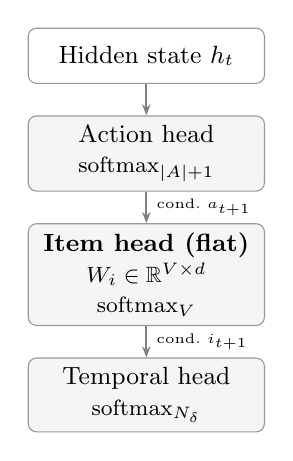
\begin{tikzpicture}[
  node distance=4mm and 8mm,
  box/.style={draw, rounded corners=3pt, minimum width=30mm,
              minimum height=7mm, font=\small, align=center,
              fill=white, draw=black!40},
  head/.style={box, fill=black!4},
  arr/.style={-{Stealth[length=4pt]}, thick, draw=black!50},
]
\node[box] (h) {Hidden state $h_t$};
\node[head, below=of h] (ah) {Action head\\\footnotesize $\mathrm{softmax}_{|A|+1}$};
\node[head, below=of ah] (ih) {\textbf{Item head (flat)}\\\footnotesize $W_i \in \mathbb{R}^{V \times d}$\\\footnotesize $\mathrm{softmax}_V$};
\node[head, below=of ih] (th) {Temporal head\\\footnotesize $\mathrm{softmax}_{N_\delta}$};
\draw[arr] (h)  -- (ah);
\draw[arr] (ah) -- node[right,font=\tiny]{cond.\ $a_{t+1}$} (ih);
\draw[arr] (ih) -- node[right,font=\tiny]{cond.\ $i_{t+1}$} (th);
\end{tikzpicture}
\caption{Iteration 1. A single $V$-way softmax predicts the SKU directly
from $h_t$, conditioned only on the sampled action.}
\label{fig:arch-iter1}
\end{figure}

\begin{figure}[H]
\centering
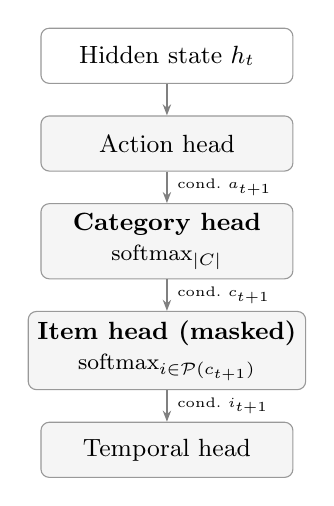
\begin{tikzpicture}[
  node distance=4mm and 8mm,
  box/.style={draw, rounded corners=3pt, minimum width=32mm,
              minimum height=7mm, font=\small, align=center,
              fill=white, draw=black!40},
  head/.style={box, fill=black!4},
  arr/.style={-{Stealth[length=4pt]}, thick, draw=black!50},
]
\node[box] (h) {Hidden state $h_t$};
\node[head, below=of h] (ah) {Action head};
\node[head, below=of ah] (ch) {\textbf{Category head}\\\footnotesize $\mathrm{softmax}_{|C|}$};
\node[head, below=of ch] (ih) {\textbf{Item head (masked)}\\\footnotesize $\mathrm{softmax}_{i \in \mathcal{P}(c_{t+1})}$};
\node[head, below=of ih] (th) {Temporal head};
\draw[arr] (h)  -- (ah);
\draw[arr] (ah) -- node[right,font=\tiny]{cond.\ $a_{t+1}$} (ch);
\draw[arr] (ch) -- node[right,font=\tiny]{cond.\ $c_{t+1}$} (ih);
\draw[arr] (ih) -- node[right,font=\tiny]{cond.\ $i_{t+1}$} (th);
\end{tikzpicture}
\caption{Iteration 2. A category head intervenes between $h_t$ and the
item softmax; the item softmax is masked to the SKU pool of the sampled
category.}
\label{fig:arch-iter2}
\end{figure}

\begin{figure}[H]
\centering
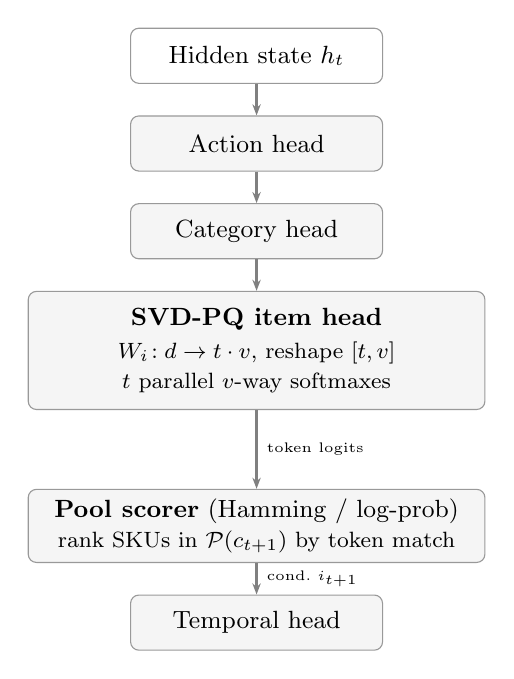
\begin{tikzpicture}[
  node distance=4mm and 6mm,
  box/.style={draw, rounded corners=3pt, minimum width=32mm,
              minimum height=7mm, font=\small, align=center,
              fill=white, draw=black!40},
  head/.style={box, fill=black!4},
  small/.style={box, minimum width=10mm, minimum height=7mm, font=\footnotesize},
  arr/.style={-{Stealth[length=4pt]}, thick, draw=black!50},
]
\node[box] (h) {Hidden state $h_t$};
\node[head, below=of h] (ah) {Action head};
\node[head, below=of ah] (ch) {Category head};
\node[head, below=of ch, minimum width=58mm, minimum height=15mm] (ih)
  {\textbf{SVD-PQ item head}\\[1pt]
   \footnotesize $W_i\!: d \to t \cdot v$, reshape $[t,v]$\\
   \footnotesize $t$ parallel $v$-way softmaxes};
\node[head, below=10mm of ih, minimum width=58mm] (sc)
  {\textbf{Pool scorer} (Hamming / log-prob)\\
   \footnotesize rank SKUs in $\mathcal{P}(c_{t+1})$ by token match};
\node[head, below=of sc] (th) {Temporal head};
\draw[arr] (h)  -- (ah);
\draw[arr] (ah) -- (ch);
\draw[arr] (ch) -- (ih);
\draw[arr] (ih) -- node[right,font=\tiny]{token logits} (sc);
\draw[arr] (sc) -- node[right,font=\tiny]{cond.\ $i_{t+1}$} (th);
\end{tikzpicture}
\caption{Iteration 3. The item head emits $t$ parallel $v$-way token
softmaxes; an offline SVD-PQ codebook maps each SKU to a token tuple, and
an in-pool scorer maps the token logits back to a single SKU at inference
time.}
\label{fig:arch-iter3}
\end{figure}

\section{Additional Experimental Details}
\label{sec:appendix-experimental}

The fidelity metric suite referenced from
Section~\ref{sec:fidelity} is reproduced in full in
Table~\ref{tab:fidelity-metrics}.

\begin{table*}[t]
\caption{Fidelity metric suite. Distributional metrics compare generated
sessions to the training distribution; behavioral-rate metrics compare
session-level event composition; bias metrics are informational and
diagnose item-side collapse against a size-matched real subsample.
Lower is better for all metrics except where indicated. All metrics are
implemented in \texttt{evaluation/fidelity.py}.}
\label{tab:fidelity-metrics}
\small
\begin{tabularx}{\textwidth}{@{}l l l X@{}}
\toprule
Group & Metric & Range & Description \\
\midrule
\multirow{5}{*}{Distributional}
  & JSD(action distribution)
    & $[0, 1]$
    & Jensen--Shannon divergence between real and generated action-type
      frequencies (5 event types). Marginal-level behavioral mix
      \cite{lin1991jsd}. \\
  & KS(session length)
    & $[0, 1]$
    & Two-sample Kolmogorov--Smirnov statistic on session length
      distributions. Engagement-shape match. \\
  & L1(action bigram matrix)
    & $[0, 2]$
    & L1 distance between normalized real and generated action bigram
      transition matrices. Sequential structure of actions, not just
      marginals. \\
  & KS(temporal $\delta_t$)
    & $[0, 1]$
    & Two-sample KS on inter-event delta-time distributions in seconds.
      Pacing realism. \\
  & Sample diversity (Jaccard ratio)
    & ratio, $1.0$ ideal
    & Mean pairwise Jaccard distance over item sets in synthetic
      sessions, normalized by the same statistic on real sessions.
      Reported as a ratio so the sparse-catalog Jaccard floor cancels;
      $<1$ means synthetic sessions are too repetitive across users,
      $>1$ means too diffuse. \\
\midrule
\multirow{2}{*}{Behavioral rate}
  & $\Delta$ conversion rate
    & $[0, 1]$
    & Absolute difference between the fraction of synthetic and real
      sessions containing at least one \texttt{product\_buy}. Funnel
      endpoint match. \\
  & $\Delta$ cart abandonment rate
    & $[0, 1]$
    & Absolute difference between the fraction of sessions containing
      \texttt{add\_to\_cart} but no \texttt{product\_buy}. Mid-funnel
      drop-off. \\
\midrule
\multirow{3}{*}{Bias (informational)}
  & Item coverage
    & ratio, $1.0$ ideal
    & Unique synthetic SKUs divided by unique SKUs in the size-matched
      real subsample. Diagnoses head-only generation. \\
  & Popularity JSD
    & $[0, 1]$
    & JSD between synthetic and matched-real per-SKU popularity
      distributions over the union of SKU keys (no top-$K$
      truncation). \\
  & $\Delta$ Gini
    & $[0, 1]$
    & Absolute difference between the Gini coefficients of the
      synthetic and matched-real SKU frequency distributions.
      Concentration parity. \\
\bottomrule
\end{tabularx}
\end{table*}

[TODO~--~full hyperparameter table, training curves, hardware utilization
notes.]

\section{Additional Results}
[TODO~--~extended fidelity tables, full transition matrices, per-seed
results, additional qualitative examples.]

\section{Demonstrator Pipeline Reference}
[TODO~--~brief reference for the configuration-driven demonstrator script:
inputs, outputs, supported generator types, sample run on a held-out
subset of the Synerise dataset.]

\end{document}